% Created 2021-06-15 Tue 18:50
% Intended LaTeX compiler: xelatex
\documentclass[xcolor=table,10pt,aspectratio=169]{beamer}
\RequirePackage{etex}
\RequirePackage[l2tabu,orthodox]{nag}            %% Warn about obsolete commands and packages
\RequirePackage{amsmath,amsfonts,amssymb,amsthm} %% Math
\RequirePackage{ifxetex,ifluatex}                %% Detect XeTeX and LuaTeX
\RequirePackage{fixltx2e}                        %% provides \textsubscript
\RequirePackage{xspace}
\RequirePackage{graphicx}
\RequirePackage{comment}
\RequirePackage{url}
\RequirePackage{relsize}
\RequirePackage{booktabs}
\RequirePackage{tabularx}
\RequirePackage[normalem]{ulem}
\RequirePackage[all]{xy}
\RequirePackage{etoolbox}

%%%
%%% Code Listings
%%%

\RequirePackage{listings}
\lstdefinelanguage{Sage}[]{Python}{morekeywords={True,False,sage,cdef,cpdef,ctypedef,self},sensitive=true}

\lstset{frame=none,
  showtabs=False,
  showspaces=False,
  showstringspaces=False,
  commentstyle={\color{gray}},
  keywordstyle={\color{mLightBrown}\textbf},
  stringstyle ={\color{mDarkBrown}},
  frame=single,
  basicstyle=\tt\scriptsize\relax,
  backgroundcolor=\color{gray!190!black},
  inputencoding=utf8,
  literate={…}{{\ldots}}1,
  belowskip=0.0em,
}

\makeatletter
\patchcmd{\@verbatim}
  {\verbatim@font}
  {\verbatim@font\scriptsize}
  {}{}
\makeatother

%%%
%%% Tikz
%%%

\RequirePackage{tikz,pgfplots}
\pgfplotsset{compat=newest}

\usetikzlibrary{calc}
\usetikzlibrary{arrows}
\usetikzlibrary{automata}
\usetikzlibrary{positioning}
\usetikzlibrary{decorations.pathmorphing}
\usetikzlibrary{backgrounds}
\usetikzlibrary{fit,}
\usetikzlibrary{shapes.symbols}
\usetikzlibrary{chains}
\usetikzlibrary{shapes.geometric}
\usetikzlibrary{shapes.arrows}
\usetikzlibrary{graphs}

%% Cache but disable by default

\usetikzlibrary{external}
\tikzexternalize[]
\tikzset{external/export=false}

%%%
%%% SVG (Inkscape)
%%%

\ifxetex % chktex 1
\providecommand{\executeiffilenewer}[3]{%
  {\immediate\write18{#3}} % hack
}
\else
\providecommand{\executeiffilenewer}[3]{%
  \ifnum\pdfstrcmp{\pdffilemoddate{#1}}%
    {\pdffilemoddate{#2}}>0%
    {\immediate\write18{#3}}
  \fi%
}
\fi

\providecommand{\includesvg}[2][1.0\textwidth]{%
 \executeiffilenewer{#1.svg}{#1.pdf}%
 {inkscape -z -D --file=#2.svg --export-pdf=#2.pdf --export-latex --export-area-page}%
 \def\svgwidth{#1} 
 \input{#2.pdf_tex}%
} 

%%%
%%% Metropolis Theme
%%%

\usetheme{metropolis}
\metroset{color/block=fill}
\metroset{numbering=none}
\metroset{outer/progressbar=foot}
\metroset{titleformat=smallcaps}

\setbeamercolor{description item}{fg=mLightBrown}
% \setbeamerfont{alerted text}{series=\bfseries}
\setbeamerfont{footnote}{size=\scriptsize}
\setbeamercolor{example text}{fg=mDarkBrown}
\setbeamercolor{block title alerted}{fg=white, bg=mDarkBrown}
\setbeamertemplate{bibliography item}[text]

\renewcommand*{\UrlFont}{\ttfamily\relax}

%%%
%%% UTF-8 & Fonts
%%% 

\RequirePackage{unicodesymbols} % after metropolis which loads fontspec

\setmonofont[BoldFont={Cousine Bold},
             ItalicFont={Cousine Italic},
             BoldItalicFont={Cousine Bold Italic},
             Scale=0.9]{Cousine}             
%%%
%%% BibLaTeX
%%%

\RequirePackage[backend=bibtex,
            style=alphabetic,
            maxnames=8,
            citestyle=alphabetic]{biblatex}

\bibliography{local.bib,abbrev3.bib,crypto_crossref.bib,rfc.bib,jacm.bib,dcc.bib}

\DeclareFieldFormat{title}{\alert{#1}}
\DeclareFieldFormat[book]{title}{\alert{#1}}
\DeclareFieldFormat[thesis]{title}{\alert{#1}}
\DeclareFieldFormat[inproceedings]{title}{\alert{#1}}
\DeclareFieldFormat[incollection]{title}{\alert{#1}}
\DeclareFieldFormat[article]{title}{\alert{#1}}
\DeclareFieldFormat[misc]{title}{\alert{#1}}

%%% 
%%% Microtype
%%%

\IfFileExists{upquote.sty}{\RequirePackage{upquote}}{}
\IfFileExists{microtype.sty}{\RequirePackage{microtype}}{}

\setlength{\parindent}{0pt}                   %%
\setlength{\parskip}{6pt plus 2pt minus 1pt}  %%
\setlength{\emergencystretch}{3em}            %% prevent overfull lines
\setcounter{secnumdepth}{0}                   %%

%%% Local Variables:
%%% mode: latex
%%% End:
\usepackage{graphicx}
\usepackage{grffile}
\usepackage{longtable}
\usepackage{wrapfig}
\usepackage{rotating}
\usepackage[normalem]{ulem}
\usepackage{amsmath}
\usepackage{textcomp}
\usepackage{amssymb}
\usepackage{capt-of}
\usepackage{hyperref}
\usepackage{microtype}
\usepackage{newunicodechar}
\usepackage[notions,operators,sets,keys,ff,adversary,primitives,complexity,asymptotics,lambda,landau,advantage]{cryptocode}
\usepackage[capitalize]{cleveref}
\usepackage{xspace}
\usepackage{units}
\usepackage{nicefrac}
\usepackage{gensymb}
\usepackage{amsthm}
\usepackage{amsmath}
\usepackage{amssymb}
\usepackage{xcolor}
\usepackage{listings}
\usepackage[color=yellow!40]{todonotes}
\DeclareMathOperator{\Vol}{Vol}
\DeclareMathOperator{\GH}{GH}
\renewcommand{\vec}[1]{\ensuremath{\mathbf{#1}}\xspace}
\renewcommand{\norm}[1]{\left\lVert#1\right\rVert}
\providecommand{\mat}[1]{\ensuremath{\vec{#1}}\xspace}
\tikzexternalize[prefix=tikz-pictures/]
\tikzset{external/optimize=false}
\tikzset{external/export=false}
\definecolor{DarkPurple}{HTML}{332288}
\definecolor{DarkBlue}{HTML}{6699CC}
\definecolor{LightBlue}{HTML}{88CCEE}
\definecolor{DarkGreen}{HTML}{117733}
\definecolor{DarkRed}{HTML}{661100}
\definecolor{LightRed}{HTML}{CC6677}
\definecolor{LightPink}{HTML}{AA4466}
\definecolor{DarkPink}{HTML}{882255}
\definecolor{LightPurple}{HTML}{AA4499}
\definecolor{DarkBrown}{HTML}{604c38}
\definecolor{DarkTeal}{HTML}{23373b}
\definecolor{LightBrown}{HTML}{EB811B}
\definecolor{LightGreen}{HTML}{14B03D}
\definecolor{DarkOrange}{HTML}{FFDD00}

\pgfplotsset{width=1.0\textwidth,
height=0.6\textwidth,
xlabel={$\beta$},
ylabel={$\log_{2}(\#\textnormal{nodes})$},
cycle list={%
solid,LightGreen,thick\\%
dotted,LightRed,very thick\\%
dashed,DarkBlue,thick\\%
dashdotted,DarkPink,thick\\%
dashdotdotted,LightGreen,thick\\%
loosely dotted,very thick\\%
loosely dashed,DarkBlue,very thick\\%
loosely dashdotted,DarkPink,very thick\\%
\\%
DarkBrown,thick\\%
},
legend pos=north west,
legend cell align={left}}

\pgfplotsset{select coords between index/.style 2 args={
x filter/.code={
\ifnum\coordindex<#1\def\pgfmathresult{}\fi
\ifnum\coordindex>#2\def\pgfmathresult{}\fi
}
}}
\usetheme{default}
\author{Martin R. Albrecht\footnote{based on joint work with Shi Bai, Pierre-Alain Fouque, Paul Kirchner, Jianwei Li, Joe Rowell, Damien Stehlé and Weiqiang Wen}}
\date{15 June 2021, Lattice Reunion}
\title{What is Lattice Point Enumeration up to These Days?}
\subtitle{… being a subroutine of BKZ}
\hypersetup{
pdfauthor={Martin R. Albrecht\footnote{based on joint work with Shi Bai, Pierre-Alain Fouque, Paul Kirchner, Jianwei Li, Joe Rowell, Damien Stehlé and Weiqiang Wen}},
pdftitle={What is Lattice Point Enumeration up to These Days?},
pdfkeywords={},
pdfsubject={},
pdfcreator={Emacs 28.0.50 (Org mode 9.4.6)},
pdflang={English},
colorlinks,
citecolor=gray,
filecolor=gray,
linkcolor=gray,
urlcolor=gray
}
\begin{document}

\maketitle
\begin{frame}{Outline}
\tableofcontents
\end{frame}


\begin{frame}[label={sec:org4b2505f}]{Headline}
\tikzset{external/export=true}
\tikzsetnextfilename{headline}
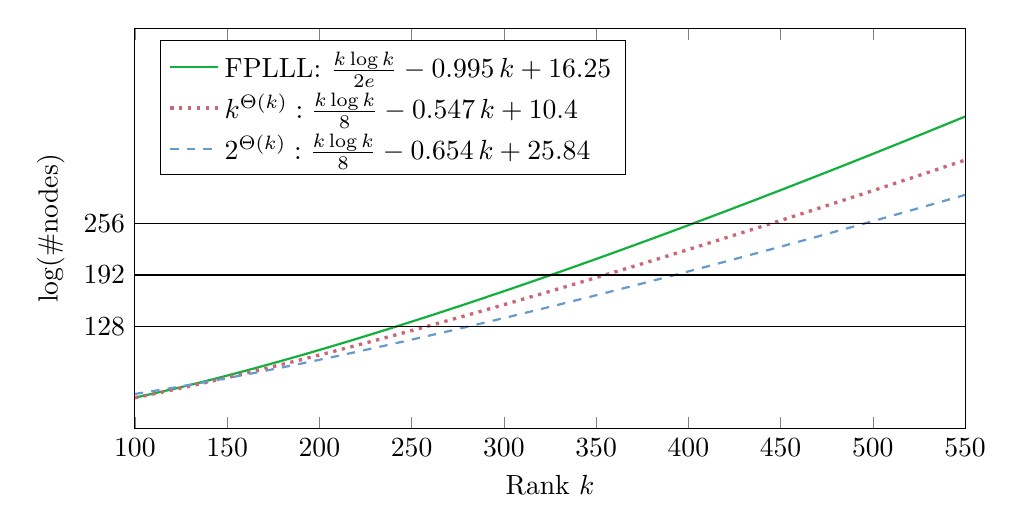
\begin{tikzpicture}
  \begin{axis}[
    legend pos = north west, 
    xlabel=Rank \(k\),
    xmin=100, xmax=550,
    ymin=0, ymax=500,
    height=0.55\textwidth,
    ylabel = \(\log(\#\textnormal{nodes})\),
    ytick = {128,192,256},
    ]
    \addplot+ [domain=100:550, samples=250]{0.1839*x*log2(x) - 0.995*x + 16.25};
    \addlegendentry{FPLLL: \(\frac{k \log k}{2e} - 0.995\,k + 16.25\)};

    \addplot+ [domain=100:550, samples=250]{0.125*x*log2(x) - 0.547*x+10.4};
    \addlegendentry{\(k^{\Theta(k)}: \frac{k \log k}{\alert{8}} - 0.547\,k + 10.4\)};

    \addplot+ [domain=100:550,samples=250]{0.125*x*log2(x) - 0.654*x+25.84};
    \addlegendentry{\(2^{\Theta(k)}: \frac{k \log k}{8} - \alert{0.654}\,k + 25.84\)};

    \addplot+ [domain=100:550, samples=200, solid, thin,draw=black]{128};
    \addplot+ [domain=100:550, samples=200, solid, thin,draw=black]{192};
    \addplot+ [domain=100:550, samples=200, solid, thin,draw=black]{256};
  \end{axis}
\end{tikzpicture}
\tikzset{external/export=false}
\end{frame}

\section{Preliminaries}
\label{sec:orga893c09}
\begin{frame}[label={sec:orgb52b206}]{Length of Gram-Schmidt Vectors}
It will be useful to consider the lengths of the Gram-Schmidt vectors.

The vector \(\vec{b}^*_i\) is the orthogonal projection of \(\vec{b}_i\) to the space spanned by the vectors \(\vec{b}_0, \ldots, \vec{b}_{i-1}\).

\begin{columns}
\begin{column}{0.45\columnwidth}
Informally, this means taking out the contributions in the directions of previous vectors  \(\vec{b}_0, \ldots, \vec{b}_{i-1}\).
\end{column}

\begin{column}{0.45\columnwidth}
\begin{tikzpicture}
\pgfplotsset{width=\textwidth, height=0.6\textwidth}
\draw[->] (0,0) -- (3,1);
\node[] at (3.2,1.2) {$\vec{b}_0$};
\only<1>{\draw[->] (0,0) -- (1,2);}
\only<1>{\node[] at (1.2,2.2) {$\vec{b}_1$};}
\only<2>{\draw[->,color=lightgray] (0,0) -- (1,2);}
\only<2>{\node[color=lightgray] at (1.2,2.2) {$\vec{b}_1$};}
\only<2>{\draw[->,gray] (0,0) -- (-0.5,1.5);}
\only<2>{\node[] at (-0.3,1.7) {$\vec{b}^*_1$};}
\only<1>{\node[] at (-0.3,1.7) {\phantom{$\vec{b}^*_1$}};}
\end{tikzpicture}
\end{column}
\end{columns}
\end{frame}

\begin{frame}[label={sec:orgdb7796f},fragile]{Example}
 \lstset{language=sage,label= ,caption= ,captionpos=b,numbers=none}
\begin{lstlisting}
sage: A = IntegerMatrix.random(120, "qary", k=60, bits=20)[::-1]
sage: M = GSO.Mat(A); M.update_gso()
sage: line([(i,log(r_, 2)/2) for i, r_ in enumerate(M.r())], **plot_kwds)
\end{lstlisting}

\begin{center}
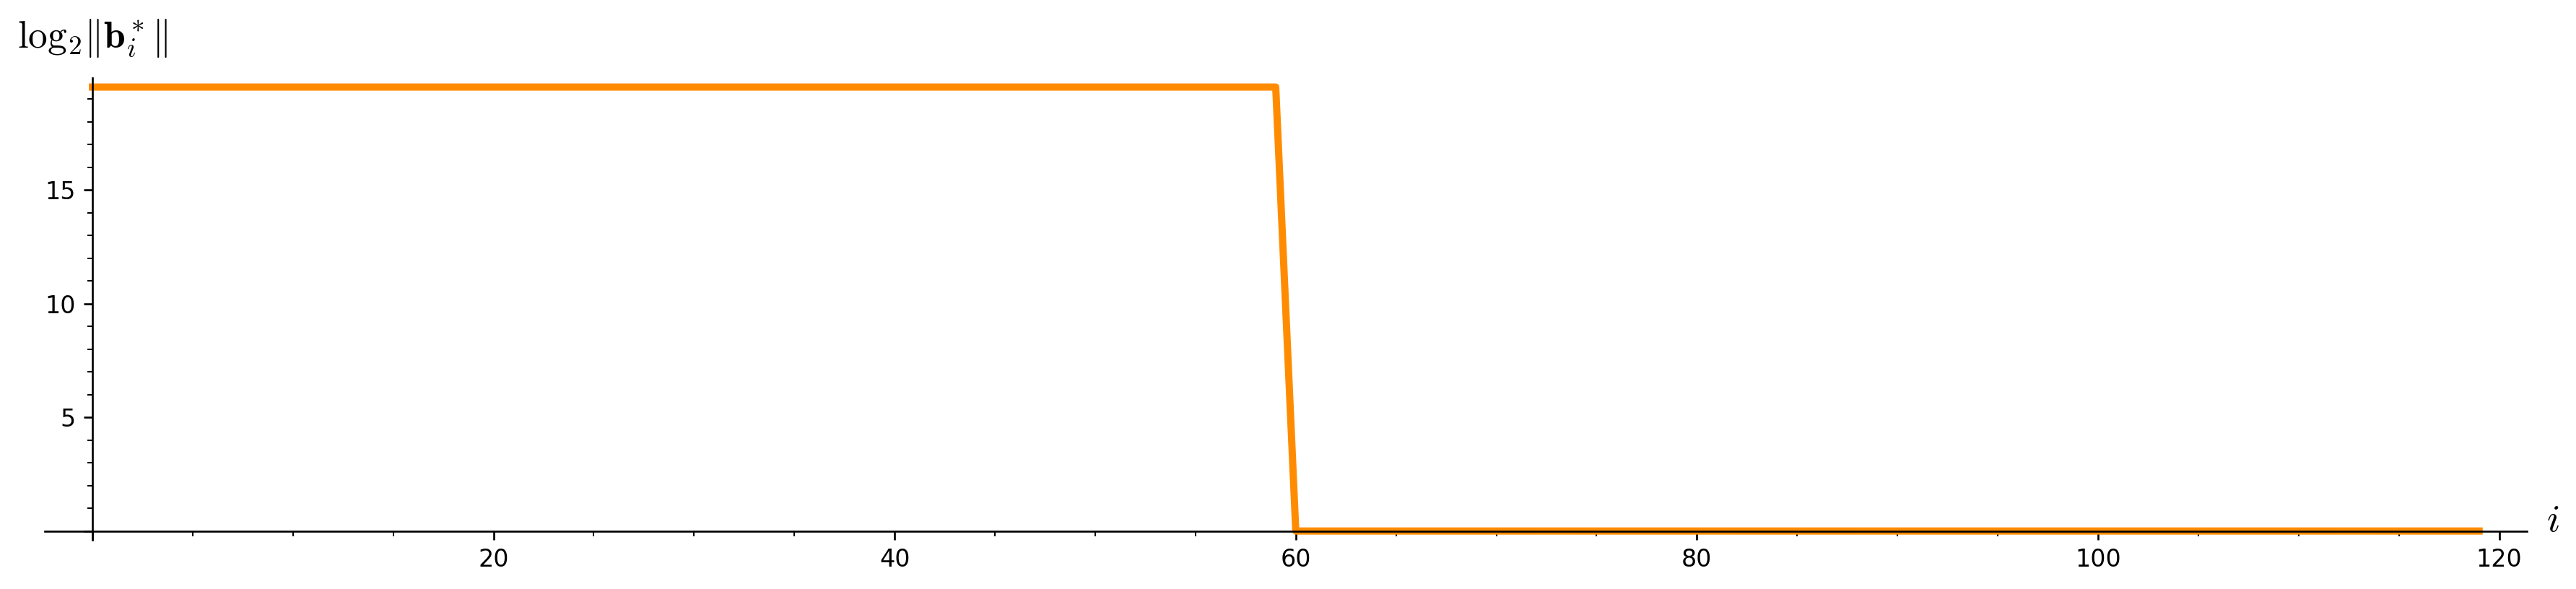
\includegraphics[width=.9\linewidth]{./gram-schmidt-norms.png}
\end{center}
\end{frame}

\begin{frame}[label={sec:org0aa2a19},fragile]{Example - LLL}
 \lstset{language=sage,label= ,caption= ,captionpos=b,numbers=none}
\begin{lstlisting}
sage: A = LLL.reduction(A)
sage: M = GSO.Mat(A); M.update_gso()
sage: line([(i,log(r_, 2)/2) for i, r_ in enumerate(M.r())], **plot_kwds)
\end{lstlisting}

\begin{center}
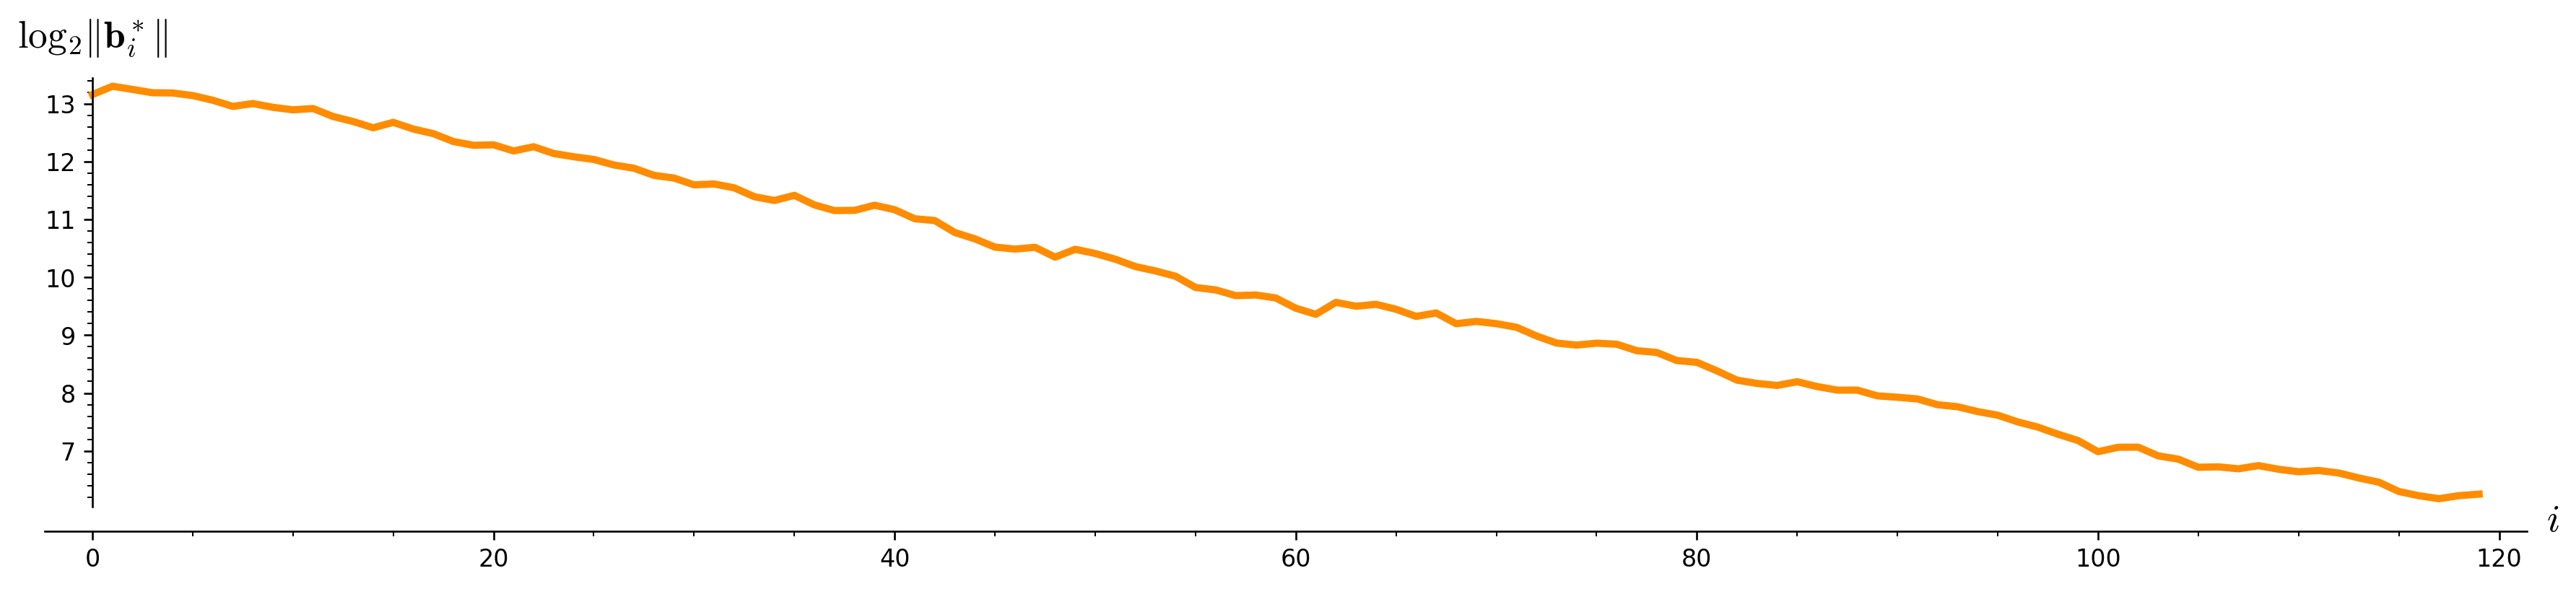
\includegraphics[width=.9\linewidth]{gram-schmidt-norms-lll.png}
\end{center}
\end{frame}

\begin{frame}[label={sec:orgb81ef7c}]{BKZ Algorithm}
\centering
\(
 \left(
     \begin{array}{ccccccccc}
                 &           &           &           &           &           &           &           &           \\
                 &           &           &           &           &           &           &           &           \\
                 &           &           &           &           &           &           &           &           \\
         \only<1-2>{\vec{b}_{0}}   \only<3->{{\color{LightRed} \vec{b}_{0}}}          &
         \only<1-5>{\vec{b}_{1}}   \only<6->{{\color{LightRed} \vec{b}_{1}}}          &
         \only<1-8>{\vec{b}_{2}}   \only<9->{{\color{LightRed} \vec{b}_{2}}}          &
         {\vec{b}_{3}}                                                             &
         {\vec{b}_{4}}                                                             &
         {\vec{b}_{5}}                                                             &
         {\vec{b}_{6}}                                                             &
         {\vec{b}_{7}}                                                             &
         \dots   \\
                 &           &           &           &           &           &           &           &           \\
                 &           &           &           &           &           &           &           &           \\
                 &           &           &           &           &           &           &           &
     \end{array}
        \right)
    \)
    \begin{tikzpicture}[remember picture, overlay]
      \tikzset{shift={(current page.center)},yshift=-1.5cm}
      \node[] at (0,0) (origin) {};
      {\color{DarkBlue} %
        \only<1-3>{%
          \draw (-.1,3) -- (-.1,2) {};
          \draw (-.1,1) -- (-.1,0) {};
          \draw (-3,3) -- (-3,2) {};
          \draw (-3,1) -- (-3,0) {};
          \draw[decorate,decoration={brace,amplitude=10pt}]
          (-3,3.2) -- (-.1,3.2) node [black,midway,yshift=.6cm]
          {$k = 5$};
          \only<2>{%
            \draw[decorate,decoration={brace,amplitude=10pt}]
            (-.1,-.2) -- (-3,-.2) {};
          }
        }
        \only<4-6>{%
          \draw (.6,3) -- (.6,2) {};
          \draw (.6,1) -- (.6,0) {};
          \draw (-2.3,3) -- (-2.3,2) {};
          \draw (-2.3,1) -- (-2.3,0) {};
          \draw[decorate,decoration={brace,amplitude=10pt}]
          (-2.3,3.2) -- (.6,3.2) node [black,midway,yshift=.6cm]
          {$k = 5$};
          \only<5>{%
            \draw[decorate,decoration={brace,amplitude=10pt}]
            (.6,-.2) -- (-2.3,-.2) {};
          }
        }
        \only<7-9>{%
          \draw (1.3,3) -- (1.3,2) {};
          \draw (1.3,1) -- (1.3,0) {};
          \draw (-1.6,3) -- (-1.6,2) {};
          \draw (-1.6,1) -- (-1.6,0) {};
          \draw[decorate,decoration={brace,amplitude=10pt}]
          (-1.6,3.2) -- (1.3,3.2) node [black,midway,yshift=.6cm]
          {$k = 5$};
          \only<8>{%
            \draw[decorate,decoration={brace,amplitude=10pt}]
            (1.3,-.2) -- (-1.6,-.2) {};
          }
        }
      }
      \node (oracle) at (-4,-1.8) {
\includegraphics[scale=0.9]{oracle.png}};
      \only<2>{%
        \draw[->] (-2.8,-.5) to[in=70,out=160] (-4,-.8);
        \draw[->] (-3,-2) to [in=270,out=20] (-0.5,-.5);
      }
      \only<5>{%
        \draw[->] (-2.1,-.5) to[in=70,out=160] (-4,-.8);
        \draw[->] (-3,-2) to [in=270,out=20] (.2,-.5);
      }
      \only<8>{%
        \draw[->] (-1.4,-.5) to[in=70,out=160] (-4,-.8);
        \draw[->] (-3,-2) to [in=270,out=20] (.2,-.5);      
      }
      \node at (5, -2.5) {\tiny{Picture credit: Eamonn Postlethwaite}};
\end{tikzpicture}
\end{frame}

\begin{frame}[label={sec:org8f01117},fragile]{BKZ Algorithm}
 \begin{columns}[t]
\begin{column}{0.4\columnwidth}
\lstset{language=Python,label= ,caption= ,captionpos=b,numbers=none}
\begin{lstlisting}
def bkz_tour(B, k, e):
    for i in range(0, e):
        preprocess(B[i:i+k])
        v = svp(B[i:i+k])
        insert(v, B, i)

 def bkz(B, k):
    while True:
        bkz_tour(B, k, d-1)
        if nothing_changed(B):
            break
\end{lstlisting}
\end{column}

\begin{column}{0.6\columnwidth}
\footnotesize

\begin{itemize}
\item \fullcite{Schnorr87}
\item \fullcite{SchEuc94}
\item \fullcite{C:HanPujSte11}
\item \fullcite{EPRINT:LiNgu20}
\end{itemize}
\end{column}
\end{columns}
\end{frame}

\begin{frame}[label={sec:org4008084},fragile]{SD-BKZ Algorithm}
 \begin{columns}[t]
\begin{column}{0.4\columnwidth}
\lstset{language=Python,label= ,caption= ,captionpos=b,numbers=none}
\begin{lstlisting}
def dual_bkz_tour(B, k, e):
    D = dual(B) # not actually needed
    for i in range(0, e):
        preprocess(D[i:i+k])
        v = svp(D[i:i+k])
        insert(v, D, i)
    B = dual(D)

 def sd_bkz(B, k):
    while True:
        bkz_tour(B, k, d-k)
        dual_bkz_tour(B, k, d-k)
        if nothing_changed(B):
            break
\end{lstlisting}
\end{column}

\begin{column}{0.6\columnwidth}
\footnotesize

\begin{itemize}
\item \fullcite{EC:MicWal16}
\end{itemize}
\end{column}
\end{columns}
\end{frame}

\begin{frame}[label={sec:org30cc5c9}]{GSA}
\begin{center}
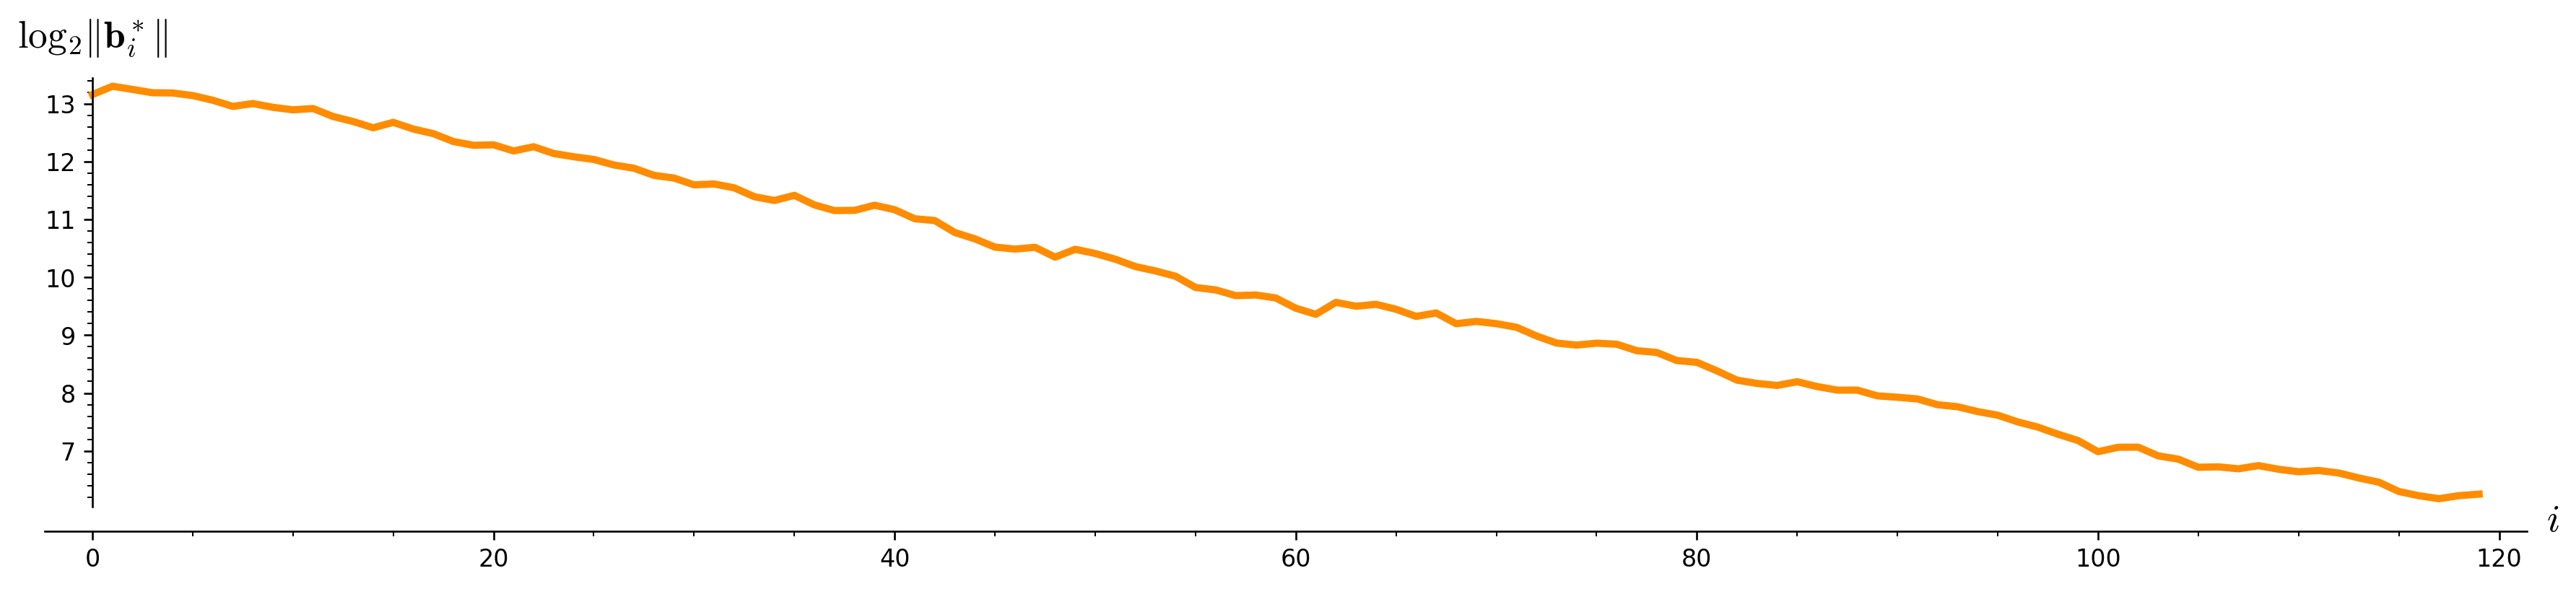
\includegraphics[width=.9\linewidth]{gram-schmidt-norms-lll.png}
\end{center}

\textbf{Geometric Series Assumption:} The shape after lattice reduction is a line with a flatter slope as lattice reduction gets stronger.\footfullcite{STACS:Schnorr03}
\end{frame}

\begin{frame}[label={sec:org4e5058d}]{Heuristics}
\begin{description}
\item[{Heuristic 1}] The GSA holds for the first \(n-k\) vectors after SD-BKZ-\(k\) reduction.
\item[{Heuristic 2}] The GSA holds.
\end{description}

\begin{block}{Scope}
Heuristics only used in theorems, our simulations make no heuristic assumptions. Our simulations are backed up by experimental evidence (in small-ish dimensions) from implementations.
\end{block}
\end{frame}

\section{Enumeration Recap}
\label{sec:orgbecb4f1}
\begin{frame}[label={sec:orgd8c22c7}]{Enumeration I -- Pick a radius}
\begin{center}
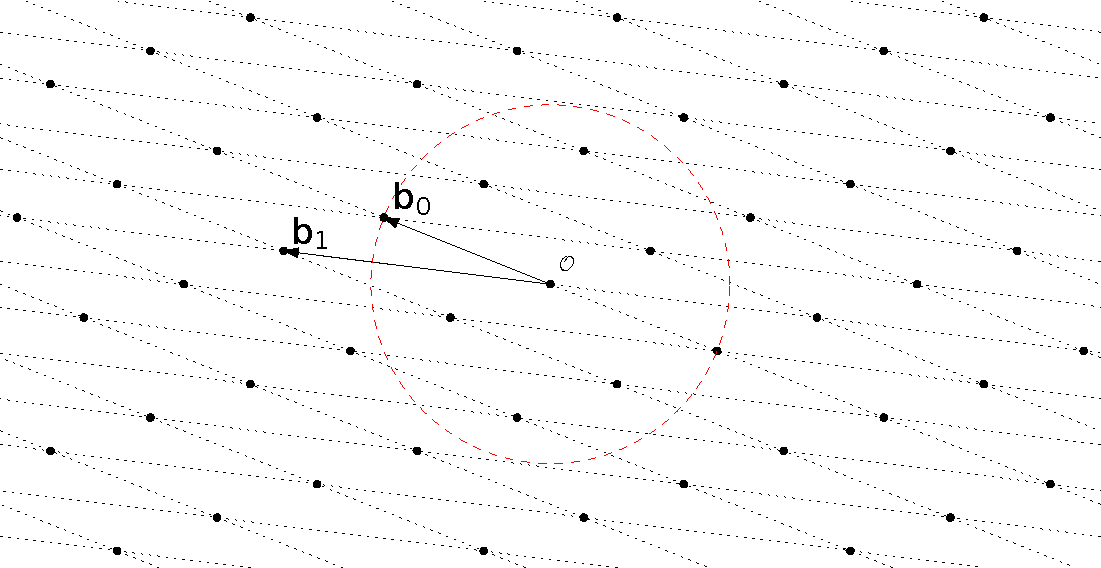
\includegraphics[width=.9\linewidth]{./joop-enum1.pdf}
\end{center}

\tiny Picture credit: Joop van de Pol
\end{frame}

\begin{frame}[label={sec:org0453286}]{Enumeration II -- Project basis}
\begin{center}
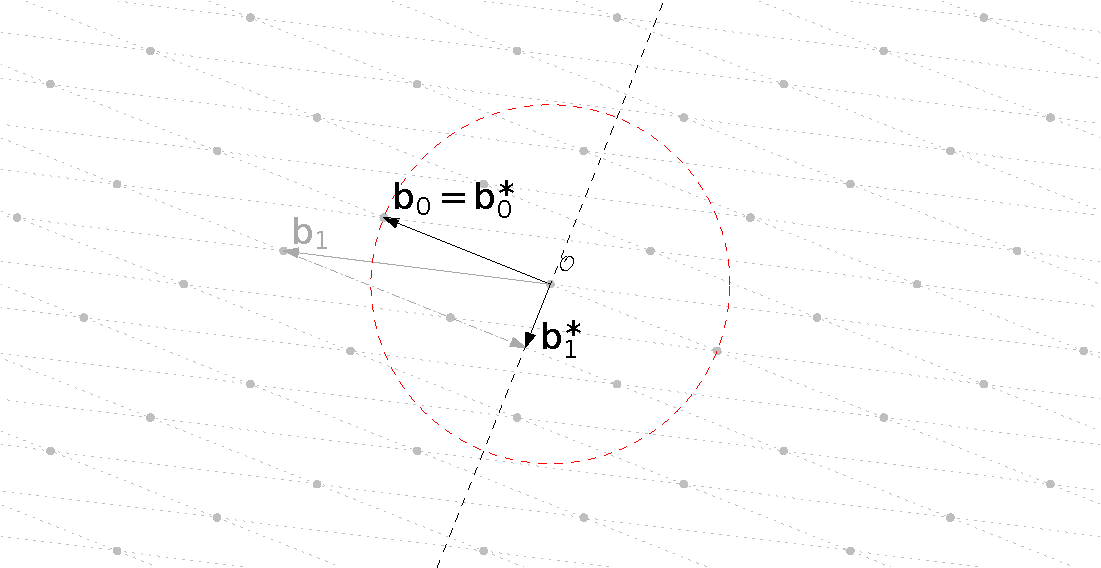
\includegraphics[width=.9\linewidth]{./joop-enum2.pdf}
\end{center}

\tiny Picture credit: Joop van de Pol
\end{frame}

\begin{frame}[label={sec:org724f1bf}]{Enumeration III -- Project lattice}
\begin{center}
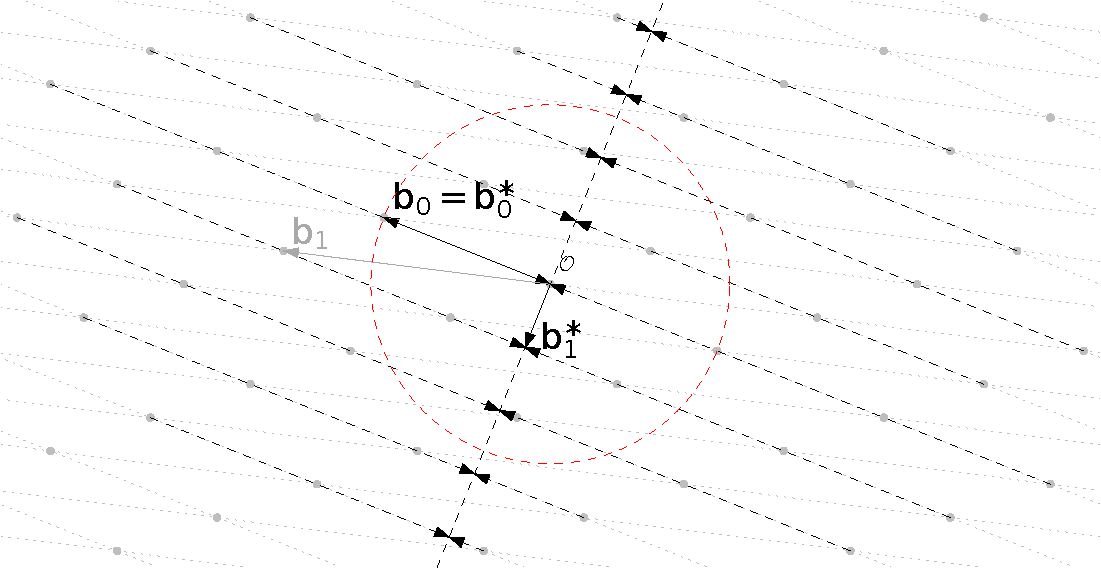
\includegraphics[width=.9\linewidth]{./joop-enum3.pdf}
\end{center}

\tiny Picture credit: Joop van de Pol
\end{frame}

\begin{frame}[label={sec:org1df0b77}]{Enumeration IV -- Enumerate projections}
\begin{center}
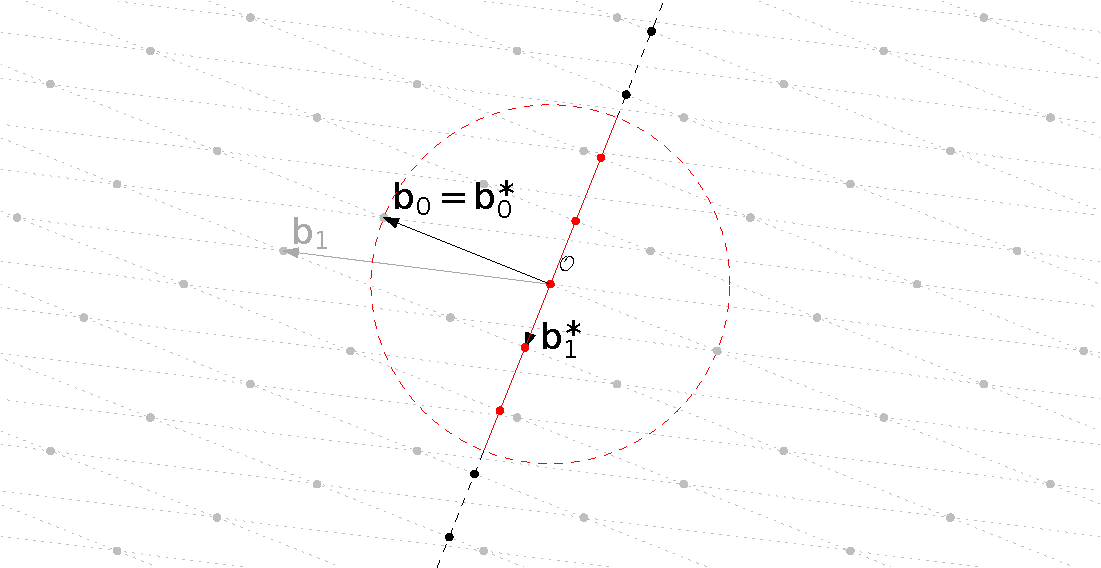
\includegraphics[width=.9\linewidth]{./joop-enum5.pdf}
\end{center}

\tiny Picture credit: Joop van de Pol
\end{frame}

\begin{frame}[label={sec:orgf01360f}]{Enumeration V -- For each lift and enumerate}
\begin{center}
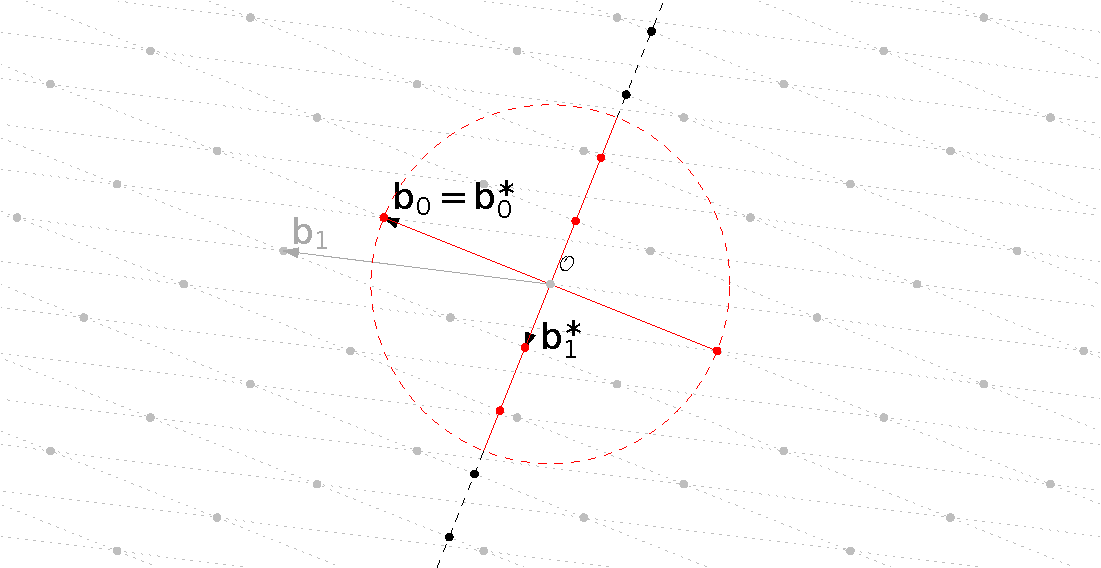
\includegraphics[width=.9\linewidth]{./joop-enum6.pdf}
\end{center}

\tiny Picture credit: Joop van de Pol
\end{frame}

\begin{frame}[label={sec:org682637a}]{Enumeration V -- For each lift and enumerate}
\begin{center}
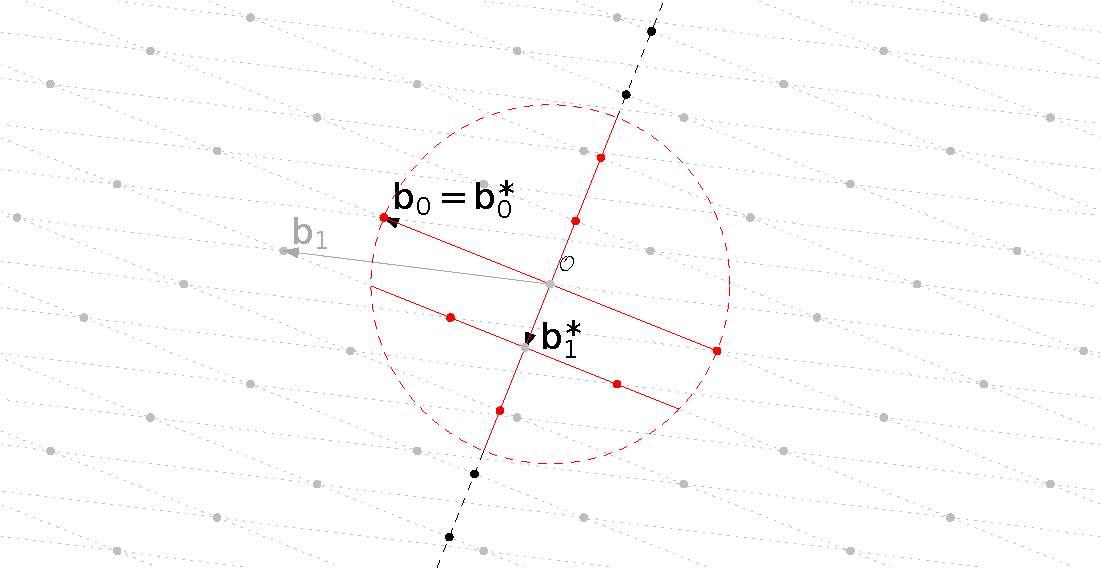
\includegraphics[width=.9\linewidth]{./joop-enum7.pdf}
\end{center}

\tiny Picture credit: Joop van de Pol
\end{frame}

\begin{frame}[label={sec:orgce1893e}]{Enumeration VI -- Keep shortest}
\begin{center}
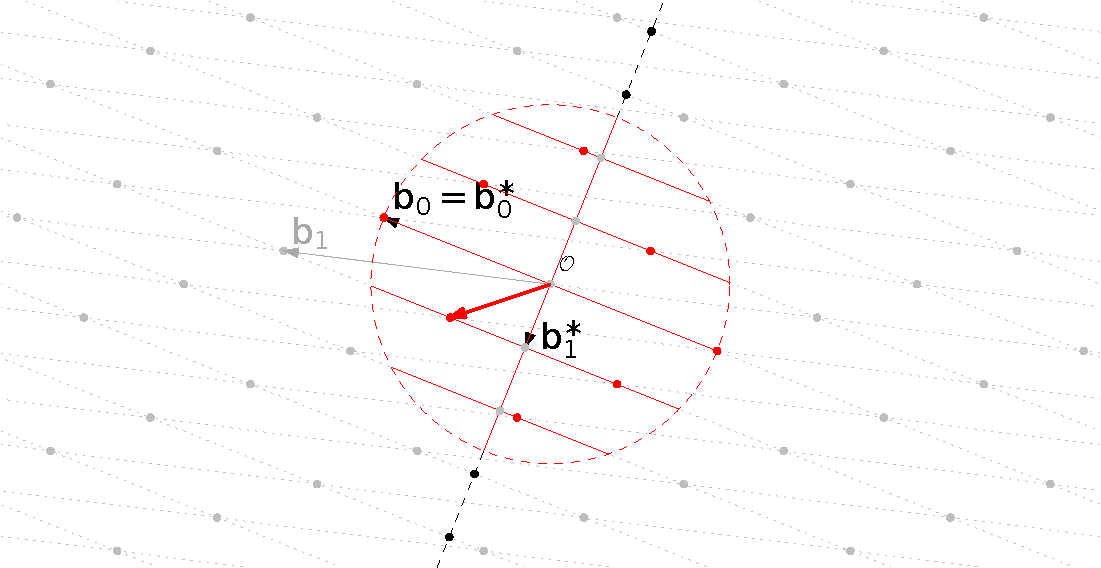
\includegraphics[width=.9\linewidth]{./joop-enum8.pdf}
\end{center}

\tiny Picture credit: Joop van de Pol
\end{frame}

\begin{frame}[label={sec:orgd2457ad}]{Enumeration Cost: \(k^{k/(2e) + o(k)}\) I}
\begin{quote}
“We obtain a new worst-case complexity upper bound, as well as the first worst-case complexity lower
bound, both of the order d of \(2^{O(d)} \cdot d^{\frac{d}{2e}}\) (up to polynomial factors) bit
operations, where \(d\) is the rank of the lattice.”\footnote{Full version of \fullcite{C:HanSte07}, available at \url{http://perso.ens-lyon.fr/damien.stehle/KANNAN\_EXTENDED.html}\label{orge03878f}}
\end{quote}
\end{frame}

\begin{frame}[label={sec:orgb875356}]{Enumeration Cost: \(k^{k/(2e) + o(k)}\) II}
\tikzset{external/export=true}
\tikzsetnextfilename{fig-fplll-costs}
\begin{tikzpicture}
  \begin{axis}[xmin=100,height=0.4\textwidth]
    \addplot table [x=d, col sep=comma, y expr = log2(\thisrowno{2})]{data/fplll-simulations,qary.csv};
    \addlegendentry{FP(y)LLL simulation};
    \addplot+ [domain=100:500, samples=250]{0.1839*x*log2(x) - 0.995*x + 16.25};
    \addlegendentry{\(1/(2e)\, k \log(k) - 0.995\cdot k + 16.25\)};
  \end{axis}
\end{tikzpicture}
\tikzset{external/export=false}

\footnotesize \fullcite{C:ABFKSW20}
\end{frame}

\section{Super-exponential: \((1+ c)\cdot k\)}
\label{sec:org67d6309}
\begin{frame}[label={sec:org1e521cb}]{Paper}
\fullcite{C:ABFKSW20}
\end{frame}

\begin{frame}[label={sec:org3ef24bc}]{Enumeration Heuristic Best-Case Complexity}
\begin{quote}
“Some authors favor the hypothesis that the average behaviour of an HKZ-reduced basis is rather a geometric decrease of the \(\|\vec{b}_i^{*}\|\)’s, i.e., roughly \(\|\vec{b}^*_i\| ≈ d^{\frac{i}{d}} \cdot \|\vec{b}_1\|\). With such a basis, solving SVP by Kannan’s algorithm would have a \(2^{O(d)} \cdot d^{\frac{d}{8}}\) complexity.”\textsuperscript{\ref{orge03878f}}
\end{quote}

\begin{alertblock}{One Interpretation}
\(\approx\) our result immediately holds if you simply assume the GSA.
\end{alertblock}
\end{frame}


\begin{frame}[label={sec:orgea47d91}]{\(1/8 = 0.125\) v \(1/(2e) \approx 0.184\)}
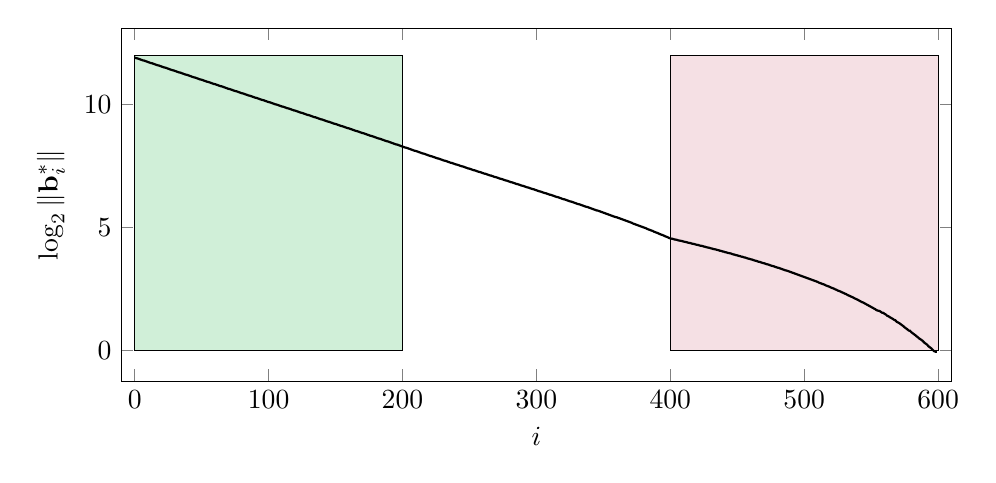
\begin{tikzpicture}
  \begin{axis}[xmin=-10, xmax=610, xlabel=\(i\),ylabel=\(\log_2 \|\vec{b}_i^*\|\),height=0.5\textwidth]
    \draw[fill=LightGreen!20!white,line width=0] (axis cs: 0,0) rectangle (axis cs: 200,12);
    \draw[fill=LightRed!20!white,line width=0] (axis cs: 400,0) rectangle (axis cs: 600,12);
    \addplot+[black] coordinates {
      (  0, 11.91) (  1, 11.89) (  2, 11.88) (  3, 11.86) (  4, 11.84) (  5, 11.82) (  6, 11.80)
      (  7, 11.79) (  8, 11.77) (  9, 11.75) ( 10, 11.73) ( 11, 11.71) ( 12, 11.69) ( 13, 11.68)
      ( 14, 11.66) ( 15, 11.64) ( 16, 11.62) ( 17, 11.60) ( 18, 11.59) ( 19, 11.57) ( 20, 11.55)
      ( 21, 11.53) ( 22, 11.51) ( 23, 11.50) ( 24, 11.48) ( 25, 11.46) ( 26, 11.44) ( 27, 11.42)
      ( 28, 11.40) ( 29, 11.39) ( 30, 11.37) ( 31, 11.35) ( 32, 11.33) ( 33, 11.31) ( 34, 11.30)
      ( 35, 11.28) ( 36, 11.26) ( 37, 11.24) ( 38, 11.22) ( 39, 11.21) ( 40, 11.19) ( 41, 11.17)
      ( 42, 11.15) ( 43, 11.13) ( 44, 11.11) ( 45, 11.10) ( 46, 11.08) ( 47, 11.06) ( 48, 11.04)
      ( 49, 11.02) ( 50, 11.01) ( 51, 10.99) ( 52, 10.97) ( 53, 10.95) ( 54, 10.93) ( 55, 10.92)
      ( 56, 10.90) ( 57, 10.88) ( 58, 10.86) ( 59, 10.84) ( 60, 10.83) ( 61, 10.81) ( 62, 10.79)
      ( 63, 10.77) ( 64, 10.75) ( 65, 10.74) ( 66, 10.72) ( 67, 10.70) ( 68, 10.68) ( 69, 10.66)
      ( 70, 10.64) ( 71, 10.63) ( 72, 10.61) ( 73, 10.59) ( 74, 10.57) ( 75, 10.55) ( 76, 10.54)
      ( 77, 10.52) ( 78, 10.50) ( 79, 10.48) ( 80, 10.46) ( 81, 10.45) ( 82, 10.43) ( 83, 10.41)
      ( 84, 10.39) ( 85, 10.37) ( 86, 10.36) ( 87, 10.34) ( 88, 10.32) ( 89, 10.30) ( 90, 10.28)
      ( 91, 10.27) ( 92, 10.25) ( 93, 10.23) ( 94, 10.21) ( 95, 10.19) ( 96, 10.18) ( 97, 10.16)
      ( 98, 10.14) ( 99, 10.12) (100, 10.10) (101, 10.09) (102, 10.07) (103, 10.05) (104, 10.03)
      (105, 10.01) (106, 10.00) (107,  9.98) (108,  9.96) (109,  9.94) (110,  9.92) (111,  9.91)
      (112,  9.89) (113,  9.87) (114,  9.85) (115,  9.84) (116,  9.82) (117,  9.80) (118,  9.78)
      (119,  9.76) (120,  9.75) (121,  9.73) (122,  9.71) (123,  9.69) (124,  9.67) (125,  9.66)
      (126,  9.64) (127,  9.62) (128,  9.60) (129,  9.58) (130,  9.57) (131,  9.55) (132,  9.53)
      (133,  9.51) (134,  9.49) (135,  9.48) (136,  9.46) (137,  9.44) (138,  9.42) (139,  9.40)
      (140,  9.39) (141,  9.37) (142,  9.35) (143,  9.33) (144,  9.31) (145,  9.30) (146,  9.28)
      (147,  9.26) (148,  9.24) (149,  9.22) (150,  9.21) (151,  9.19) (152,  9.17) (153,  9.15)
      (154,  9.13) (155,  9.12) (156,  9.10) (157,  9.08) (158,  9.06) (159,  9.04) (160,  9.03)
      (161,  9.01) (162,  8.99) (163,  8.97) (164,  8.95) (165,  8.93) (166,  8.92) (167,  8.90)
      (168,  8.88) (169,  8.86) (170,  8.84) (171,  8.83) (172,  8.81) (173,  8.79) (174,  8.77)
      (175,  8.75) (176,  8.73) (177,  8.72) (178,  8.70) (179,  8.68) (180,  8.66) (181,  8.64)
      (182,  8.62) (183,  8.61) (184,  8.59) (185,  8.57) (186,  8.55) (187,  8.53) (188,  8.51)
      (189,  8.50) (190,  8.48) (191,  8.46) (192,  8.44) (193,  8.42) (194,  8.40) (195,  8.38)
      (196,  8.37) (197,  8.35) (198,  8.33) (199,  8.31) (200,  8.29) (201,  8.27) (202,  8.25)
      (203,  8.24) (204,  8.22) (205,  8.20) (206,  8.18) (207,  8.16) (208,  8.14) (209,  8.12)
      (210,  8.11) (211,  8.09) (212,  8.07) (213,  8.05) (214,  8.03) (215,  8.01) (216,  8.00)
      (217,  7.98) (218,  7.96) (219,  7.94) (220,  7.92) (221,  7.90) (222,  7.89) (223,  7.87)
      (224,  7.85) (225,  7.83) (226,  7.81) (227,  7.80) (228,  7.78) (229,  7.76) (230,  7.74)
      (231,  7.72) (232,  7.71) (233,  7.69) (234,  7.67) (235,  7.65) (236,  7.63) (237,  7.62)
      (238,  7.60) (239,  7.58) (240,  7.56) (241,  7.55) (242,  7.53) (243,  7.51) (244,  7.49)
      (245,  7.48) (246,  7.46) (247,  7.44) (248,  7.42) (249,  7.40) (250,  7.39) (251,  7.37)
      (252,  7.35) (253,  7.33) (254,  7.32) (255,  7.30) (256,  7.28) (257,  7.26) (258,  7.25)
      (259,  7.23) (260,  7.21) (261,  7.19) (262,  7.18) (263,  7.16) (264,  7.14) (265,  7.12)
      (266,  7.11) (267,  7.09) (268,  7.07) (269,  7.05) (270,  7.04) (271,  7.02) (272,  7.00)
      (273,  6.98) (274,  6.97) (275,  6.95) (276,  6.93) (277,  6.91) (278,  6.90) (279,  6.88)
      (280,  6.86) (281,  6.84) (282,  6.83) (283,  6.81) (284,  6.79) (285,  6.77) (286,  6.76)
      (287,  6.74) (288,  6.72) (289,  6.70) (290,  6.69) (291,  6.67) (292,  6.65) (293,  6.63)
      (294,  6.62) (295,  6.60) (296,  6.58) (297,  6.56) (298,  6.55) (299,  6.53) (300,  6.51)
      (301,  6.49) (302,  6.47) (303,  6.46) (304,  6.44) (305,  6.42) (306,  6.40) (307,  6.39)
      (308,  6.37) (309,  6.35) (310,  6.33) (311,  6.32) (312,  6.30) (313,  6.28) (314,  6.26)
      (315,  6.24) (316,  6.23) (317,  6.21) (318,  6.19) (319,  6.17) (320,  6.15) (321,  6.14)
      (322,  6.12) (323,  6.10) (324,  6.08) (325,  6.06) (326,  6.05) (327,  6.03) (328,  6.01)
      (329,  5.99) (330,  5.97) (331,  5.95) (332,  5.94) (333,  5.92) (334,  5.90) (335,  5.88)
      (336,  5.86) (337,  5.84) (338,  5.83) (339,  5.81) (340,  5.79) (341,  5.77) (342,  5.75)
      (343,  5.73) (344,  5.71) (345,  5.69) (346,  5.68) (347,  5.66) (348,  5.64) (349,  5.62)
      (350,  5.60) (351,  5.58) (352,  5.56) (353,  5.54) (354,  5.52) (355,  5.50) (356,  5.48)
      (357,  5.46) (358,  5.44) (359,  5.42) (360,  5.41) (361,  5.39) (362,  5.37) (363,  5.35)
      (364,  5.33) (365,  5.31) (366,  5.29) (367,  5.27) (368,  5.25) (369,  5.23) (370,  5.21)
      (371,  5.19) (372,  5.16) (373,  5.14) (374,  5.12) (375,  5.10) (376,  5.08) (377,  5.06)
      (378,  5.04) (379,  5.02) (380,  5.00) (381,  4.98) (382,  4.96) (383,  4.93) (384,  4.91)
      (385,  4.89) (386,  4.87) (387,  4.85) (388,  4.82) (389,  4.80) (390,  4.78) (391,  4.76)
      (392,  4.73) (393,  4.71) (394,  4.69) (395,  4.67) (396,  4.64) (397,  4.62) (398,  4.60)
      (399,  4.57) (400,  4.55) (401,  4.54) (402,  4.53) (403,  4.51) (404,  4.50) (405,  4.49)
      (406,  4.47) (407,  4.46) (408,  4.45) (409,  4.44) (410,  4.42) (411,  4.41) (412,  4.40)
      (413,  4.38) (414,  4.37) (415,  4.36) (416,  4.34) (417,  4.33) (418,  4.32) (419,  4.30)
      (420,  4.29) (421,  4.28) (422,  4.26) (423,  4.25) (424,  4.24) (425,  4.22) (426,  4.21)
      (427,  4.19) (428,  4.18) (429,  4.17) (430,  4.15) (431,  4.14) (432,  4.12) (433,  4.11)
      (434,  4.10) (435,  4.08) (436,  4.07) (437,  4.05) (438,  4.04) (439,  4.02) (440,  4.01)
      (441,  3.99) (442,  3.98) (443,  3.96) (444,  3.95) (445,  3.94) (446,  3.92) (447,  3.90)
      (448,  3.89) (449,  3.87) (450,  3.86) (451,  3.84) (452,  3.83) (453,  3.81) (454,  3.80)
      (455,  3.78) (456,  3.77) (457,  3.75) (458,  3.73) (459,  3.72) (460,  3.70) (461,  3.69)
      (462,  3.67) (463,  3.65) (464,  3.64) (465,  3.62) (466,  3.60) (467,  3.59) (468,  3.57)
      (469,  3.55) (470,  3.54) (471,  3.52) (472,  3.50) (473,  3.49) (474,  3.47) (475,  3.45)
      (476,  3.43) (477,  3.42) (478,  3.40) (479,  3.38) (480,  3.36) (481,  3.35) (482,  3.33)
      (483,  3.31) (484,  3.29) (485,  3.27) (486,  3.25) (487,  3.24) (488,  3.22) (489,  3.20)
      (490,  3.18) (491,  3.16) (492,  3.14) (493,  3.12) (494,  3.10) (495,  3.08) (496,  3.06)
      (497,  3.04) (498,  3.02) (499,  3.00) (500,  2.98) (501,  2.96) (502,  2.94) (503,  2.92)
      (504,  2.90) (505,  2.88) (506,  2.86) (507,  2.84) (508,  2.82) (509,  2.80) (510,  2.78)
      (511,  2.75) (512,  2.73) (513,  2.71) (514,  2.69) (515,  2.67) (516,  2.64) (517,  2.62)
      (518,  2.60) (519,  2.58) (520,  2.55) (521,  2.53) (522,  2.51) (523,  2.48) (524,  2.46)
      (525,  2.43) (526,  2.41) (527,  2.39) (528,  2.36) (529,  2.34) (530,  2.31) (531,  2.29)
      (532,  2.26) (533,  2.23) (534,  2.21) (535,  2.18) (536,  2.16) (537,  2.13) (538,  2.10)
      (539,  2.08) (540,  2.05) (541,  2.02) (542,  1.99) (543,  1.96) (544,  1.94) (545,  1.91)
      (546,  1.88) (547,  1.85) (548,  1.82) (549,  1.79) (550,  1.76) (551,  1.73) (552,  1.70)
      (553,  1.67) (554,  1.63) (555,  1.61) (556,  1.60) (557,  1.57) (558,  1.53) (559,  1.52)
      (560,  1.48) (561,  1.45) (562,  1.40) (563,  1.38) (564,  1.34) (565,  1.31) (566,  1.28)
      (567,  1.24) (568,  1.22) (569,  1.16) (570,  1.13) (571,  1.10) (572,  1.06) (573,  1.02)
      (574,  0.98) (575,  0.93) (576,  0.89) (577,  0.85) (578,  0.80) (579,  0.79) (580,  0.73)
      (581,  0.69) (582,  0.65) (583,  0.61) (584,  0.56) (585,  0.52) (586,  0.47) (587,  0.44)
      (588,  0.40) (589,  0.35) (590,  0.29) (591,  0.26) (592,  0.21) (593,  0.15) (594,  0.11)
      (595,  0.07) (596,  0.01) (597, -0.04) (598, -0.06) (599, -0.06) 
    };
  \end{axis}
\end{tikzpicture}
\end{frame}

\begin{frame}[label={sec:orga5c8622}]{Why we can’t have Nice Things}
\begin{enumerate}
\item We run enumeration many times each succeeding with low probability of success and re-randomise in between: this destroys the nice GSA-line shape
\begin{itemize}
\item Thus, before enumerating a local block, we run some local preprocessing with some block size \(k' < k\)
\end{itemize}
\item In the sandpile model,\footfullcite{C:HanPujSte11} as the algorithm proceeds through the indices \(i\), a “bump” accumulates from index \(i + 1\) onward.
\end{enumerate}
\end{frame}

\begin{frame}[label={sec:orgd16aa76}]{Idea: Overshoot Preprocessing}
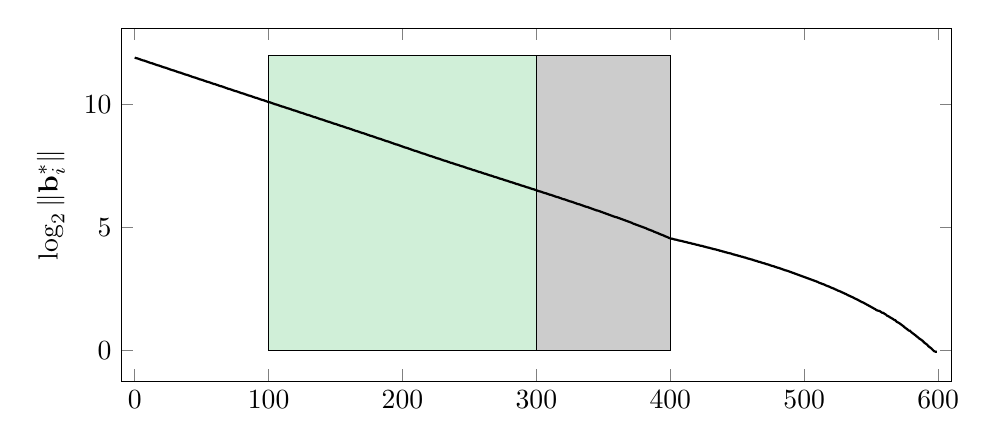
\begin{tikzpicture}
  \begin{axis}[xmin=-10, xmax=610, xlabel=,ylabel=\(\log_2 \|\vec{b}_i^*\|\),height=0.5\textwidth]
    \draw[fill=black!20!white,line width=0] (axis cs: 100,0) rectangle (axis cs: 400,12);
    \draw[fill=LightGreen!20!white,line width=0] (axis cs: 100,0) rectangle (axis cs: 300,12);
    \addplot+[black] coordinates {
      (  0, 11.91) (  1, 11.89) (  2, 11.88) (  3, 11.86) (  4, 11.84) (  5, 11.82) (  6, 11.80)
      (  7, 11.79) (  8, 11.77) (  9, 11.75) ( 10, 11.73) ( 11, 11.71) ( 12, 11.69) ( 13, 11.68)
      ( 14, 11.66) ( 15, 11.64) ( 16, 11.62) ( 17, 11.60) ( 18, 11.59) ( 19, 11.57) ( 20, 11.55)
      ( 21, 11.53) ( 22, 11.51) ( 23, 11.50) ( 24, 11.48) ( 25, 11.46) ( 26, 11.44) ( 27, 11.42)
      ( 28, 11.40) ( 29, 11.39) ( 30, 11.37) ( 31, 11.35) ( 32, 11.33) ( 33, 11.31) ( 34, 11.30)
      ( 35, 11.28) ( 36, 11.26) ( 37, 11.24) ( 38, 11.22) ( 39, 11.21) ( 40, 11.19) ( 41, 11.17)
      ( 42, 11.15) ( 43, 11.13) ( 44, 11.11) ( 45, 11.10) ( 46, 11.08) ( 47, 11.06) ( 48, 11.04)
      ( 49, 11.02) ( 50, 11.01) ( 51, 10.99) ( 52, 10.97) ( 53, 10.95) ( 54, 10.93) ( 55, 10.92)
      ( 56, 10.90) ( 57, 10.88) ( 58, 10.86) ( 59, 10.84) ( 60, 10.83) ( 61, 10.81) ( 62, 10.79)
      ( 63, 10.77) ( 64, 10.75) ( 65, 10.74) ( 66, 10.72) ( 67, 10.70) ( 68, 10.68) ( 69, 10.66)
      ( 70, 10.64) ( 71, 10.63) ( 72, 10.61) ( 73, 10.59) ( 74, 10.57) ( 75, 10.55) ( 76, 10.54)
      ( 77, 10.52) ( 78, 10.50) ( 79, 10.48) ( 80, 10.46) ( 81, 10.45) ( 82, 10.43) ( 83, 10.41)
      ( 84, 10.39) ( 85, 10.37) ( 86, 10.36) ( 87, 10.34) ( 88, 10.32) ( 89, 10.30) ( 90, 10.28)
      ( 91, 10.27) ( 92, 10.25) ( 93, 10.23) ( 94, 10.21) ( 95, 10.19) ( 96, 10.18) ( 97, 10.16)
      ( 98, 10.14) ( 99, 10.12) (100, 10.10) (101, 10.09) (102, 10.07) (103, 10.05) (104, 10.03)
      (105, 10.01) (106, 10.00) (107,  9.98) (108,  9.96) (109,  9.94) (110,  9.92) (111,  9.91)
      (112,  9.89) (113,  9.87) (114,  9.85) (115,  9.84) (116,  9.82) (117,  9.80) (118,  9.78)
      (119,  9.76) (120,  9.75) (121,  9.73) (122,  9.71) (123,  9.69) (124,  9.67) (125,  9.66)
      (126,  9.64) (127,  9.62) (128,  9.60) (129,  9.58) (130,  9.57) (131,  9.55) (132,  9.53)
      (133,  9.51) (134,  9.49) (135,  9.48) (136,  9.46) (137,  9.44) (138,  9.42) (139,  9.40)
      (140,  9.39) (141,  9.37) (142,  9.35) (143,  9.33) (144,  9.31) (145,  9.30) (146,  9.28)
      (147,  9.26) (148,  9.24) (149,  9.22) (150,  9.21) (151,  9.19) (152,  9.17) (153,  9.15)
      (154,  9.13) (155,  9.12) (156,  9.10) (157,  9.08) (158,  9.06) (159,  9.04) (160,  9.03)
      (161,  9.01) (162,  8.99) (163,  8.97) (164,  8.95) (165,  8.93) (166,  8.92) (167,  8.90)
      (168,  8.88) (169,  8.86) (170,  8.84) (171,  8.83) (172,  8.81) (173,  8.79) (174,  8.77)
      (175,  8.75) (176,  8.73) (177,  8.72) (178,  8.70) (179,  8.68) (180,  8.66) (181,  8.64)
      (182,  8.62) (183,  8.61) (184,  8.59) (185,  8.57) (186,  8.55) (187,  8.53) (188,  8.51)
      (189,  8.50) (190,  8.48) (191,  8.46) (192,  8.44) (193,  8.42) (194,  8.40) (195,  8.38)
      (196,  8.37) (197,  8.35) (198,  8.33) (199,  8.31) (200,  8.29) (201,  8.27) (202,  8.25)
      (203,  8.24) (204,  8.22) (205,  8.20) (206,  8.18) (207,  8.16) (208,  8.14) (209,  8.12)
      (210,  8.11) (211,  8.09) (212,  8.07) (213,  8.05) (214,  8.03) (215,  8.01) (216,  8.00)
      (217,  7.98) (218,  7.96) (219,  7.94) (220,  7.92) (221,  7.90) (222,  7.89) (223,  7.87)
      (224,  7.85) (225,  7.83) (226,  7.81) (227,  7.80) (228,  7.78) (229,  7.76) (230,  7.74)
      (231,  7.72) (232,  7.71) (233,  7.69) (234,  7.67) (235,  7.65) (236,  7.63) (237,  7.62)
      (238,  7.60) (239,  7.58) (240,  7.56) (241,  7.55) (242,  7.53) (243,  7.51) (244,  7.49)
      (245,  7.48) (246,  7.46) (247,  7.44) (248,  7.42) (249,  7.40) (250,  7.39) (251,  7.37)
      (252,  7.35) (253,  7.33) (254,  7.32) (255,  7.30) (256,  7.28) (257,  7.26) (258,  7.25)
      (259,  7.23) (260,  7.21) (261,  7.19) (262,  7.18) (263,  7.16) (264,  7.14) (265,  7.12)
      (266,  7.11) (267,  7.09) (268,  7.07) (269,  7.05) (270,  7.04) (271,  7.02) (272,  7.00)
      (273,  6.98) (274,  6.97) (275,  6.95) (276,  6.93) (277,  6.91) (278,  6.90) (279,  6.88)
      (280,  6.86) (281,  6.84) (282,  6.83) (283,  6.81) (284,  6.79) (285,  6.77) (286,  6.76)
      (287,  6.74) (288,  6.72) (289,  6.70) (290,  6.69) (291,  6.67) (292,  6.65) (293,  6.63)
      (294,  6.62) (295,  6.60) (296,  6.58) (297,  6.56) (298,  6.55) (299,  6.53) (300,  6.51)
      (301,  6.49) (302,  6.47) (303,  6.46) (304,  6.44) (305,  6.42) (306,  6.40) (307,  6.39)
      (308,  6.37) (309,  6.35) (310,  6.33) (311,  6.32) (312,  6.30) (313,  6.28) (314,  6.26)
      (315,  6.24) (316,  6.23) (317,  6.21) (318,  6.19) (319,  6.17) (320,  6.15) (321,  6.14)
      (322,  6.12) (323,  6.10) (324,  6.08) (325,  6.06) (326,  6.05) (327,  6.03) (328,  6.01)
      (329,  5.99) (330,  5.97) (331,  5.95) (332,  5.94) (333,  5.92) (334,  5.90) (335,  5.88)
      (336,  5.86) (337,  5.84) (338,  5.83) (339,  5.81) (340,  5.79) (341,  5.77) (342,  5.75)
      (343,  5.73) (344,  5.71) (345,  5.69) (346,  5.68) (347,  5.66) (348,  5.64) (349,  5.62)
      (350,  5.60) (351,  5.58) (352,  5.56) (353,  5.54) (354,  5.52) (355,  5.50) (356,  5.48)
      (357,  5.46) (358,  5.44) (359,  5.42) (360,  5.41) (361,  5.39) (362,  5.37) (363,  5.35)
      (364,  5.33) (365,  5.31) (366,  5.29) (367,  5.27) (368,  5.25) (369,  5.23) (370,  5.21)
      (371,  5.19) (372,  5.16) (373,  5.14) (374,  5.12) (375,  5.10) (376,  5.08) (377,  5.06)
      (378,  5.04) (379,  5.02) (380,  5.00) (381,  4.98) (382,  4.96) (383,  4.93) (384,  4.91)
      (385,  4.89) (386,  4.87) (387,  4.85) (388,  4.82) (389,  4.80) (390,  4.78) (391,  4.76)
      (392,  4.73) (393,  4.71) (394,  4.69) (395,  4.67) (396,  4.64) (397,  4.62) (398,  4.60)
      (399,  4.57) (400,  4.55) (401,  4.54) (402,  4.53) (403,  4.51) (404,  4.50) (405,  4.49)
      (406,  4.47) (407,  4.46) (408,  4.45) (409,  4.44) (410,  4.42) (411,  4.41) (412,  4.40)
      (413,  4.38) (414,  4.37) (415,  4.36) (416,  4.34) (417,  4.33) (418,  4.32) (419,  4.30)
      (420,  4.29) (421,  4.28) (422,  4.26) (423,  4.25) (424,  4.24) (425,  4.22) (426,  4.21)
      (427,  4.19) (428,  4.18) (429,  4.17) (430,  4.15) (431,  4.14) (432,  4.12) (433,  4.11)
      (434,  4.10) (435,  4.08) (436,  4.07) (437,  4.05) (438,  4.04) (439,  4.02) (440,  4.01)
      (441,  3.99) (442,  3.98) (443,  3.96) (444,  3.95) (445,  3.94) (446,  3.92) (447,  3.90)
      (448,  3.89) (449,  3.87) (450,  3.86) (451,  3.84) (452,  3.83) (453,  3.81) (454,  3.80)
      (455,  3.78) (456,  3.77) (457,  3.75) (458,  3.73) (459,  3.72) (460,  3.70) (461,  3.69)
      (462,  3.67) (463,  3.65) (464,  3.64) (465,  3.62) (466,  3.60) (467,  3.59) (468,  3.57)
      (469,  3.55) (470,  3.54) (471,  3.52) (472,  3.50) (473,  3.49) (474,  3.47) (475,  3.45)
      (476,  3.43) (477,  3.42) (478,  3.40) (479,  3.38) (480,  3.36) (481,  3.35) (482,  3.33)
      (483,  3.31) (484,  3.29) (485,  3.27) (486,  3.25) (487,  3.24) (488,  3.22) (489,  3.20)
      (490,  3.18) (491,  3.16) (492,  3.14) (493,  3.12) (494,  3.10) (495,  3.08) (496,  3.06)
      (497,  3.04) (498,  3.02) (499,  3.00) (500,  2.98) (501,  2.96) (502,  2.94) (503,  2.92)
      (504,  2.90) (505,  2.88) (506,  2.86) (507,  2.84) (508,  2.82) (509,  2.80) (510,  2.78)
      (511,  2.75) (512,  2.73) (513,  2.71) (514,  2.69) (515,  2.67) (516,  2.64) (517,  2.62)
      (518,  2.60) (519,  2.58) (520,  2.55) (521,  2.53) (522,  2.51) (523,  2.48) (524,  2.46)
      (525,  2.43) (526,  2.41) (527,  2.39) (528,  2.36) (529,  2.34) (530,  2.31) (531,  2.29)
      (532,  2.26) (533,  2.23) (534,  2.21) (535,  2.18) (536,  2.16) (537,  2.13) (538,  2.10)
      (539,  2.08) (540,  2.05) (541,  2.02) (542,  1.99) (543,  1.96) (544,  1.94) (545,  1.91)
      (546,  1.88) (547,  1.85) (548,  1.82) (549,  1.79) (550,  1.76) (551,  1.73) (552,  1.70)
      (553,  1.67) (554,  1.63) (555,  1.61) (556,  1.60) (557,  1.57) (558,  1.53) (559,  1.52)
      (560,  1.48) (561,  1.45) (562,  1.40) (563,  1.38) (564,  1.34) (565,  1.31) (566,  1.28)
      (567,  1.24) (568,  1.22) (569,  1.16) (570,  1.13) (571,  1.10) (572,  1.06) (573,  1.02)
      (574,  0.98) (575,  0.93) (576,  0.89) (577,  0.85) (578,  0.80) (579,  0.79) (580,  0.73)
      (581,  0.69) (582,  0.65) (583,  0.61) (584,  0.56) (585,  0.52) (586,  0.47) (587,  0.44)
      (588,  0.40) (589,  0.35) (590,  0.29) (591,  0.26) (592,  0.21) (593,  0.15) (594,  0.11)
      (595,  0.07) (596,  0.01) (597, -0.04) (598, -0.06) (599, -0.06) 
    };
  \end{axis}
\end{tikzpicture}

\begin{center}
Preprocessing in dimension \((1+c)\cdot k\) for enumeration in dimension \(k\).
\end{center}
\end{frame}

\begin{frame}[label={sec:orgaff36a8}]{Theorem}
\begin{theorem}[Informal]
Under Heuristic 1 there exists an algorithm that achieves root Hermite factor \(k^{{\frac{1}{2k}}}\) in time \(k^{{k/8 + o(k)}}\).
\end{theorem}

\begin{itemize}
\item Heuristic 1: The GSA holds for the first \(n-k\) vectors after SD-BKZ-\(k\) reduction.
\item Approach:
\begin{itemize}
\item Define \(k_0 = x_0 \cdot k\) with \(x_0 = \frac{e}{4}(1+o(1))\) and, for all \(i\geq 1\):
\[k_i = \lceil x_i \cdot k \rceil \ \mbox{ with } \ x_i = x_{i-1} + \sqrt{\frac{x_{i-1}}{i}}.\]
\item so we start with \(k_0^{k_{0}/(2e)} \approx k^{k/8}\)
\item preprocess with increasing block sizes \(k_{i}\)
\item enumerate over the "line" part of the shape only
\end{itemize}
\end{itemize}
\end{frame}

\begin{frame}[label={sec:org35b5780}]{Practical Performance (Simulation)}
\tikzset{external/export=true}
\tikzsetnextfilename{fig-super-exponential-performance}
\begin{tikzpicture}
  \begin{axis}[xlabel=\(k\),height=0.5\textwidth]
    \addplot+ [domain=100:500, samples=250]{0.1839*x*log2(x) - 0.995*x + 16.25};
    \addlegendentry{\(1/(2e)\, k \log(k) - 0.995\cdot k + 16.25\)};

    \addplot table [x=d, col sep=comma, y expr = log2(\thisrowno{2}), , select coords between index={0}{500}]{data/fplll-block-simulations,qary,0.25.csv};
    \addlegendentry{simulation};

    \addplot+ [domain=20:500, samples=100]{0.125*x*log2(x) + -0.547*x + 10.4};
    \addlegendentry{\(1/8\,k\log(k) - 0.547k + 10.4\) for \(c=1/4\)}
  \end{axis}
\end{tikzpicture}
\tikzset{external/export=false}
\end{frame}

\begin{frame}[label={sec:orgcfba54a}]{Not-so-extreme Pruning}
\tikzset{external/export=true}
\tikzsetnextfilename{fig-enumeration-cost-asvp-probability}
\begin{tikzpicture}
  \begin{axis}[ylabel=,legend pos=south west,height=0.4\textwidth,xlabel={$k$},]

    \addplot+ [domain=50:500, samples=500]
    {-0.09*x + 3.30};
    \addlegendentry{\(-0.09\, n + 3.30\)};

    \addplot
    table [x=d, col sep=comma, y expr = log2(\thisrow{probability})]
    {data/fplll-block-simulations,qary,0.25.csv};
    \addlegendentry{simulation};        
  \end{axis}
\end{tikzpicture}
\tikzset{external/export=false}

\begin{center}
Success probability of a single enumeration in log scale.
\end{center}
\end{frame}

\begin{frame}[label={sec:org14eadf4}]{Can we do better?}
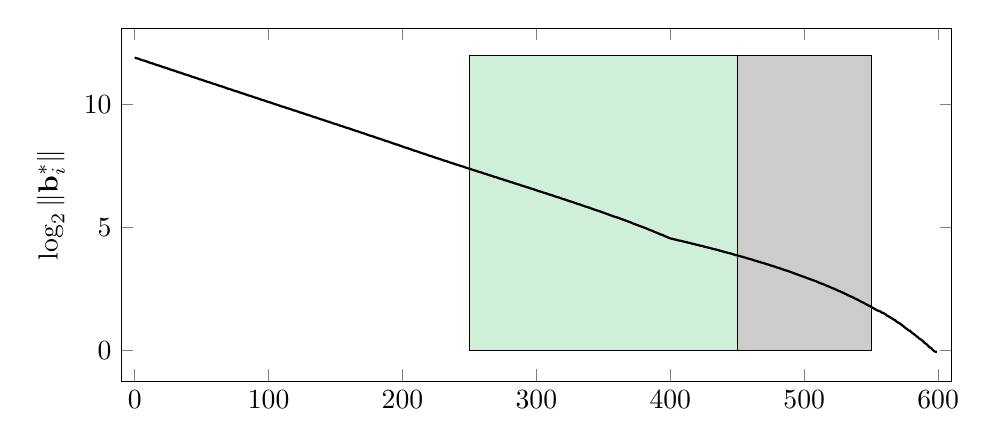
\begin{tikzpicture}
  \begin{axis}[xmin=-10, xmax=610, xlabel=,ylabel=\(\log_2 \|\vec{b}_i^*\|\),height=0.5\textwidth]
    \draw[fill=black!20!white,line width=0] (axis cs: 250,0) rectangle (axis cs: 550,12);
    \draw[fill=LightGreen!20!white,line width=0] (axis cs: 250,0) rectangle (axis cs: 450,12);
    \addplot+[black] coordinates {
      (  0, 11.91) (  1, 11.89) (  2, 11.88) (  3, 11.86) (  4, 11.84) (  5, 11.82) (  6, 11.80)
      (  7, 11.79) (  8, 11.77) (  9, 11.75) ( 10, 11.73) ( 11, 11.71) ( 12, 11.69) ( 13, 11.68)
      ( 14, 11.66) ( 15, 11.64) ( 16, 11.62) ( 17, 11.60) ( 18, 11.59) ( 19, 11.57) ( 20, 11.55)
      ( 21, 11.53) ( 22, 11.51) ( 23, 11.50) ( 24, 11.48) ( 25, 11.46) ( 26, 11.44) ( 27, 11.42)
      ( 28, 11.40) ( 29, 11.39) ( 30, 11.37) ( 31, 11.35) ( 32, 11.33) ( 33, 11.31) ( 34, 11.30)
      ( 35, 11.28) ( 36, 11.26) ( 37, 11.24) ( 38, 11.22) ( 39, 11.21) ( 40, 11.19) ( 41, 11.17)
      ( 42, 11.15) ( 43, 11.13) ( 44, 11.11) ( 45, 11.10) ( 46, 11.08) ( 47, 11.06) ( 48, 11.04)
      ( 49, 11.02) ( 50, 11.01) ( 51, 10.99) ( 52, 10.97) ( 53, 10.95) ( 54, 10.93) ( 55, 10.92)
      ( 56, 10.90) ( 57, 10.88) ( 58, 10.86) ( 59, 10.84) ( 60, 10.83) ( 61, 10.81) ( 62, 10.79)
      ( 63, 10.77) ( 64, 10.75) ( 65, 10.74) ( 66, 10.72) ( 67, 10.70) ( 68, 10.68) ( 69, 10.66)
      ( 70, 10.64) ( 71, 10.63) ( 72, 10.61) ( 73, 10.59) ( 74, 10.57) ( 75, 10.55) ( 76, 10.54)
      ( 77, 10.52) ( 78, 10.50) ( 79, 10.48) ( 80, 10.46) ( 81, 10.45) ( 82, 10.43) ( 83, 10.41)
      ( 84, 10.39) ( 85, 10.37) ( 86, 10.36) ( 87, 10.34) ( 88, 10.32) ( 89, 10.30) ( 90, 10.28)
      ( 91, 10.27) ( 92, 10.25) ( 93, 10.23) ( 94, 10.21) ( 95, 10.19) ( 96, 10.18) ( 97, 10.16)
      ( 98, 10.14) ( 99, 10.12) (100, 10.10) (101, 10.09) (102, 10.07) (103, 10.05) (104, 10.03)
      (105, 10.01) (106, 10.00) (107,  9.98) (108,  9.96) (109,  9.94) (110,  9.92) (111,  9.91)
      (112,  9.89) (113,  9.87) (114,  9.85) (115,  9.84) (116,  9.82) (117,  9.80) (118,  9.78)
      (119,  9.76) (120,  9.75) (121,  9.73) (122,  9.71) (123,  9.69) (124,  9.67) (125,  9.66)
      (126,  9.64) (127,  9.62) (128,  9.60) (129,  9.58) (130,  9.57) (131,  9.55) (132,  9.53)
      (133,  9.51) (134,  9.49) (135,  9.48) (136,  9.46) (137,  9.44) (138,  9.42) (139,  9.40)
      (140,  9.39) (141,  9.37) (142,  9.35) (143,  9.33) (144,  9.31) (145,  9.30) (146,  9.28)
      (147,  9.26) (148,  9.24) (149,  9.22) (150,  9.21) (151,  9.19) (152,  9.17) (153,  9.15)
      (154,  9.13) (155,  9.12) (156,  9.10) (157,  9.08) (158,  9.06) (159,  9.04) (160,  9.03)
      (161,  9.01) (162,  8.99) (163,  8.97) (164,  8.95) (165,  8.93) (166,  8.92) (167,  8.90)
      (168,  8.88) (169,  8.86) (170,  8.84) (171,  8.83) (172,  8.81) (173,  8.79) (174,  8.77)
      (175,  8.75) (176,  8.73) (177,  8.72) (178,  8.70) (179,  8.68) (180,  8.66) (181,  8.64)
      (182,  8.62) (183,  8.61) (184,  8.59) (185,  8.57) (186,  8.55) (187,  8.53) (188,  8.51)
      (189,  8.50) (190,  8.48) (191,  8.46) (192,  8.44) (193,  8.42) (194,  8.40) (195,  8.38)
      (196,  8.37) (197,  8.35) (198,  8.33) (199,  8.31) (200,  8.29) (201,  8.27) (202,  8.25)
      (203,  8.24) (204,  8.22) (205,  8.20) (206,  8.18) (207,  8.16) (208,  8.14) (209,  8.12)
      (210,  8.11) (211,  8.09) (212,  8.07) (213,  8.05) (214,  8.03) (215,  8.01) (216,  8.00)
      (217,  7.98) (218,  7.96) (219,  7.94) (220,  7.92) (221,  7.90) (222,  7.89) (223,  7.87)
      (224,  7.85) (225,  7.83) (226,  7.81) (227,  7.80) (228,  7.78) (229,  7.76) (230,  7.74)
      (231,  7.72) (232,  7.71) (233,  7.69) (234,  7.67) (235,  7.65) (236,  7.63) (237,  7.62)
      (238,  7.60) (239,  7.58) (240,  7.56) (241,  7.55) (242,  7.53) (243,  7.51) (244,  7.49)
      (245,  7.48) (246,  7.46) (247,  7.44) (248,  7.42) (249,  7.40) (250,  7.39) (251,  7.37)
      (252,  7.35) (253,  7.33) (254,  7.32) (255,  7.30) (256,  7.28) (257,  7.26) (258,  7.25)
      (259,  7.23) (260,  7.21) (261,  7.19) (262,  7.18) (263,  7.16) (264,  7.14) (265,  7.12)
      (266,  7.11) (267,  7.09) (268,  7.07) (269,  7.05) (270,  7.04) (271,  7.02) (272,  7.00)
      (273,  6.98) (274,  6.97) (275,  6.95) (276,  6.93) (277,  6.91) (278,  6.90) (279,  6.88)
      (280,  6.86) (281,  6.84) (282,  6.83) (283,  6.81) (284,  6.79) (285,  6.77) (286,  6.76)
      (287,  6.74) (288,  6.72) (289,  6.70) (290,  6.69) (291,  6.67) (292,  6.65) (293,  6.63)
      (294,  6.62) (295,  6.60) (296,  6.58) (297,  6.56) (298,  6.55) (299,  6.53) (300,  6.51)
      (301,  6.49) (302,  6.47) (303,  6.46) (304,  6.44) (305,  6.42) (306,  6.40) (307,  6.39)
      (308,  6.37) (309,  6.35) (310,  6.33) (311,  6.32) (312,  6.30) (313,  6.28) (314,  6.26)
      (315,  6.24) (316,  6.23) (317,  6.21) (318,  6.19) (319,  6.17) (320,  6.15) (321,  6.14)
      (322,  6.12) (323,  6.10) (324,  6.08) (325,  6.06) (326,  6.05) (327,  6.03) (328,  6.01)
      (329,  5.99) (330,  5.97) (331,  5.95) (332,  5.94) (333,  5.92) (334,  5.90) (335,  5.88)
      (336,  5.86) (337,  5.84) (338,  5.83) (339,  5.81) (340,  5.79) (341,  5.77) (342,  5.75)
      (343,  5.73) (344,  5.71) (345,  5.69) (346,  5.68) (347,  5.66) (348,  5.64) (349,  5.62)
      (350,  5.60) (351,  5.58) (352,  5.56) (353,  5.54) (354,  5.52) (355,  5.50) (356,  5.48)
      (357,  5.46) (358,  5.44) (359,  5.42) (360,  5.41) (361,  5.39) (362,  5.37) (363,  5.35)
      (364,  5.33) (365,  5.31) (366,  5.29) (367,  5.27) (368,  5.25) (369,  5.23) (370,  5.21)
      (371,  5.19) (372,  5.16) (373,  5.14) (374,  5.12) (375,  5.10) (376,  5.08) (377,  5.06)
      (378,  5.04) (379,  5.02) (380,  5.00) (381,  4.98) (382,  4.96) (383,  4.93) (384,  4.91)
      (385,  4.89) (386,  4.87) (387,  4.85) (388,  4.82) (389,  4.80) (390,  4.78) (391,  4.76)
      (392,  4.73) (393,  4.71) (394,  4.69) (395,  4.67) (396,  4.64) (397,  4.62) (398,  4.60)
      (399,  4.57) (400,  4.55) (401,  4.54) (402,  4.53) (403,  4.51) (404,  4.50) (405,  4.49)
      (406,  4.47) (407,  4.46) (408,  4.45) (409,  4.44) (410,  4.42) (411,  4.41) (412,  4.40)
      (413,  4.38) (414,  4.37) (415,  4.36) (416,  4.34) (417,  4.33) (418,  4.32) (419,  4.30)
      (420,  4.29) (421,  4.28) (422,  4.26) (423,  4.25) (424,  4.24) (425,  4.22) (426,  4.21)
      (427,  4.19) (428,  4.18) (429,  4.17) (430,  4.15) (431,  4.14) (432,  4.12) (433,  4.11)
      (434,  4.10) (435,  4.08) (436,  4.07) (437,  4.05) (438,  4.04) (439,  4.02) (440,  4.01)
      (441,  3.99) (442,  3.98) (443,  3.96) (444,  3.95) (445,  3.94) (446,  3.92) (447,  3.90)
      (448,  3.89) (449,  3.87) (450,  3.86) (451,  3.84) (452,  3.83) (453,  3.81) (454,  3.80)
      (455,  3.78) (456,  3.77) (457,  3.75) (458,  3.73) (459,  3.72) (460,  3.70) (461,  3.69)
      (462,  3.67) (463,  3.65) (464,  3.64) (465,  3.62) (466,  3.60) (467,  3.59) (468,  3.57)
      (469,  3.55) (470,  3.54) (471,  3.52) (472,  3.50) (473,  3.49) (474,  3.47) (475,  3.45)
      (476,  3.43) (477,  3.42) (478,  3.40) (479,  3.38) (480,  3.36) (481,  3.35) (482,  3.33)
      (483,  3.31) (484,  3.29) (485,  3.27) (486,  3.25) (487,  3.24) (488,  3.22) (489,  3.20)
      (490,  3.18) (491,  3.16) (492,  3.14) (493,  3.12) (494,  3.10) (495,  3.08) (496,  3.06)
      (497,  3.04) (498,  3.02) (499,  3.00) (500,  2.98) (501,  2.96) (502,  2.94) (503,  2.92)
      (504,  2.90) (505,  2.88) (506,  2.86) (507,  2.84) (508,  2.82) (509,  2.80) (510,  2.78)
      (511,  2.75) (512,  2.73) (513,  2.71) (514,  2.69) (515,  2.67) (516,  2.64) (517,  2.62)
      (518,  2.60) (519,  2.58) (520,  2.55) (521,  2.53) (522,  2.51) (523,  2.48) (524,  2.46)
      (525,  2.43) (526,  2.41) (527,  2.39) (528,  2.36) (529,  2.34) (530,  2.31) (531,  2.29)
      (532,  2.26) (533,  2.23) (534,  2.21) (535,  2.18) (536,  2.16) (537,  2.13) (538,  2.10)
      (539,  2.08) (540,  2.05) (541,  2.02) (542,  1.99) (543,  1.96) (544,  1.94) (545,  1.91)
      (546,  1.88) (547,  1.85) (548,  1.82) (549,  1.79) (550,  1.76) (551,  1.73) (552,  1.70)
      (553,  1.67) (554,  1.63) (555,  1.61) (556,  1.60) (557,  1.57) (558,  1.53) (559,  1.52)
      (560,  1.48) (561,  1.45) (562,  1.40) (563,  1.38) (564,  1.34) (565,  1.31) (566,  1.28)
      (567,  1.24) (568,  1.22) (569,  1.16) (570,  1.13) (571,  1.10) (572,  1.06) (573,  1.02)
      (574,  0.98) (575,  0.93) (576,  0.89) (577,  0.85) (578,  0.80) (579,  0.79) (580,  0.73)
      (581,  0.69) (582,  0.65) (583,  0.61) (584,  0.56) (585,  0.52) (586,  0.47) (587,  0.44)
      (588,  0.40) (589,  0.35) (590,  0.29) (591,  0.26) (592,  0.21) (593,  0.15) (594,  0.11)
      (595,  0.07) (596,  0.01) (597, -0.04) (598, -0.06) (599, -0.06) 
    };
  \end{axis}
\end{tikzpicture}
\end{frame}

\begin{frame}[label={sec:org102510e}]{Can we do better?}
\tikzset{external/export=true}
\tikzsetnextfilename{fig-hypothetical-bkz-cost}
\begin{tikzpicture}
  \begin{axis}[
    xlabel={$c$},
    legend pos=north east,
    ylabel={Interpolated constant},
    y tick label style={/pgf/number format/fixed, /pgf/number format/precision=4, /pgf/number format/fixed zerofill},
    ytick={0.125,0.1839},
    ymin=0.08, ymax=0.200,
    height=0.4\textwidth,
    ]
    \addplot table[x index=0,y index=1] {data/c-simulations.csv};
    \addlegendentry{BKZ};      
    \addplot table[x index=0,y index=2] {data/c-simulations.csv};      
    \addlegendentry{SDBKZ};
  \end{axis}
\end{tikzpicture}
\tikzset{external/export=false}

\begin{center}
Leading constant assuming \textbf{free preprocessing}.
\end{center}
\end{frame}

\section{Exponential: \({\left(\alpha \cdot \GH(k_{{\alpha}})\right)}^{\frac{1}{k_{\alpha}-1}} \leq {\GH(k)}^{\frac{1}{k-1}}\)}
\label{sec:orge42d956}
\begin{frame}[label={sec:orgb1d0105}]{Paper}
\fullcite{EPRINT:ABLR20}, to appear at CRYPTO'21.
\end{frame}

\begin{frame}[label={sec:org55eac12}]{\(\alpha \cdot GH(k)\) v \(GH(k)\)}
\begin{corollary} Let \(\Lambda\) be a full-rank lattice in \(\RR^{n}\). Let \(\alpha \ge 1\) and \(\rho \in (0, \frac{1}{2})\) such that \(4\alpha^{4}\rho(1-\rho) < 1\). Let \(R =\GH(\Lambda)\), \(R_{\alpha} =\alpha \cdot \GH(\Lambda)\) and \(f(i)\) be a certain pruning function.

Under Heuristic 2, the time complexity of enumeration with radius \(R_{\alpha}\) is less than that with radius \(R\) by a multiplicative factor \(\alpha^{n/2}\) (up to some polynomial factor).
\end{corollary} 

Corollary of Theorem 6 in \fullcite{EPRINT:LiNgu20}.
\end{frame}

\begin{frame}[label={sec:org68cce3d}]{Idea: \({\left(\alpha \cdot \GH(k_{{\alpha}})\right)}^{\frac{1}{k_{\alpha}-1}} \leq {\GH(k)}^{\frac{1}{k-1}}\)}
\tikzset{external/export=true}%
\tikzsetnextfilename{fig-ka-evolution}
\begin{tikzpicture}
  \begin{axis}[legend pos=north east,legend columns=3,
    legend style={/tikz/column 2/.style={column sep=15pt,},/tikz/column 4/.style={column sep=15pt,},},
    xlabel= \(k\),
    xmin=80, xmax=400, height=0.4\textwidth,
    ylabel = \(\frac{k_{\alpha}}{k}\),
    ytick = {1.05,1.2,1.5,1.8}
    ]
    \addplot table[x=k,y expr=\thisrow{k alpha}/\thisrow{k},col sep=comma]%
    {data/approx-hsvp-simulations,qary,1.40,0.00,1.00.csv};
    \addlegendentry{\(\alpha=1.40\)};

    \addplot table[x=k,y expr=\thisrow{k alpha}/\thisrow{k},col sep=comma]%
    {data/approx-hsvp-simulations,qary,1.30,0.00,1.00.csv};
    \addlegendentry{\(\alpha=1.30\)};

    \addplot table[x=k,y expr=\thisrow{k alpha}/\thisrow{k},col sep=comma]%
    {data/approx-hsvp-simulations,qary,1.20,0.00,1.00.csv};
    \addlegendentry{\(\alpha=1.20\)};

    \addplot table[x=k,y expr=\thisrow{k alpha}/\thisrow{k},col sep=comma]%
    {data/approx-hsvp-simulations,qary,1.10,0.00,1.00.csv};
    \addlegendentry{\(\alpha=1.10\)};

    \addplot table[x=k,y expr=\thisrow{k alpha}/\thisrow{k},col sep=comma]%
    {data/approx-hsvp-simulations,qary,1.05,0.00,1.00.csv};
    \addlegendentry{\(\alpha=1.05\)};
  \end{axis}
\end{tikzpicture}%
\tikzset{external/export=false}%

\(k_{\alpha}\) is the smallest integer greater than \(k\) such that \(\GH{(k)}^{\frac{1}{k-1}}\ge {(\alpha \cdot \GH(k_{\alpha}))}^{\frac{1}{k_{\alpha}-1}}\) for \(\alpha \geq 1\) and \(k\geq 36\).
\end{frame}

\begin{frame}[label={sec:orgb644173}]{Theorem}
\begin{theorem}[Informal]
Let \(\alpha > 1\) and \(\rho \in (0, \frac{1}{2})\) be constants such that \(4\,\alpha^{4}\,\rho\cdot (1-\rho) < 1\). Let  \(f(i)\) be a certain pruning function. Assume Heuristic 2 holds.

Let \(T(n):=n^{c_{0}n}\cdot 2^{c_{1}n}\) be the cost of enumeration. Let \(k\) a sufficiently large integer.
For any real  \(\eta \in [\frac{2\ln k}{\ln k-\ln(2\pi e^{2})},\frac{1}{2c_{0}})\), if \(1<  \alpha \le (k^{c_{0}}\cdot 2^{c_{1}})^{2}\), then some \((\alpha\cdot\GH(k_{\alpha}))\)-HSVP enumeration oracle in rank \(k_{\alpha}\)  is exponentially faster than some \(\GH(k)\)-HSVP enumeration oracle in rank \(k\) 
by a multiplicative factor of at least \[\alpha^{\left(\frac{1}{2}-c_{0}\eta\right)k}\cdot \left(4(1-\rho)\left(\frac{\sqrt{\alpha}}{{(2e)}^{c_{0}}\,2^{c_{1}}}\right)^{4\eta}\right)^{\frac{k \log \alpha}{4\log k}} \textnormal{ (up to some polynomial factor)}.\]
\end{theorem}
\end{frame}

\begin{frame}[label={sec:org4a82362}]{Practical Performance (Simulation)}
\tikzset{external/export=true}
\tikzsetnextfilename{fig-enumeration-cost-direct-k-prebest-15}
\begin{tikzpicture}
  \begin{axis}[legend pos=north west,legend columns=2,
    legend style={/tikz/column 2/.style={column sep=15pt,},},
    xlabel=Rank \(k\),
    xmin=100, xmax=400, ymin=20,ymax=240,height=0.35\textwidth,
    ]
    \addplot table[x=k,y=log(total cost),col sep=comma]%
    {data/approx-hsvp-simulations,qary,1.00,0.15,best.csv};
    \addlegendentry{\(\alpha=1.00\)};

    \addplot table[x=k,y=log(total cost),col sep=comma]%
    {data/approx-hsvp-simulations,qary,1.10,0.15,best.csv};
    \addlegendentry{\(\alpha=1.10\)};

    \addplot table[x=k,y=log(total cost),col sep=comma]%
    {data/approx-hsvp-simulations,qary,1.20,0.15,best.csv};
    \addlegendentry{\(\alpha=1.20\)};

  \end{axis}
\end{tikzpicture}
\tikzset{external/export=false}

Expected cost \(t_{\alpha}(k_{\alpha})\) of the \((\alpha\cdot\GH(k_{\alpha}))\)-HSVP enumeration oracle in rank \(k_{\alpha}\) for reaching RHF \(\GH{(k)}^{\frac{1}{k-1}}\).
\end{frame}

\begin{frame}[label={sec:orgacf2e38}]{Not-so-extreme Pruning}
\tikzset{external/export=true}
\tikzsetnextfilename{fig-relaxed-pruning}
\begin{tikzpicture}
  \begin{axis}[legend pos=south west,legend columns=2,
    legend style={
      /tikz/column 1/.style={column sep=5pt,},
      /tikz/column 2/.style={column sep=5pt,},
      /tikz/column 3/.style={column sep=5pt,},
    },
    ylabel=\(\log(\tau)\),
    xlabel=\(k\),
    xmin=100, xmax=440,
    height=0.45\textwidth,
    ]

    \addplot table[x=k,y expr=log2(\thisrow{solutions}),col sep=comma]%
    {data/approx-hsvp-simulations,qary,1.05,0.15,best.csv};
    \addlegendentry{\(\alpha=1.05\)};

    \addplot table[x=k,y expr=log2(\thisrow{solutions}),col sep=comma]%
    {data/approx-hsvp-simulations,qary,1.10,0.15,best.csv};
    \addlegendentry{\(\alpha=1.10\)};

    \addplot table[x=k,y expr=log2(\thisrow{solutions}),col sep=comma]%
    {data/approx-hsvp-simulations,qary,1.20,0.15,best.csv};
    \addlegendentry{\(\alpha=1.20\)};

    \addplot table[x=k,y expr=log2(\thisrow{solutions}),col sep=comma]%
    {data/approx-hsvp-simulations,qary,1.30,0.15,best.csv};
    \addlegendentry{\(\alpha=1.30\)};
  \end{axis}
\end{tikzpicture}
\tikzset{external/export=false}

Expected number of solutions \(\tau\) per enumeration for reaching RHF \(\GH{(k)}^{\frac{1}{k-1}}\).
\end{frame}

\begin{frame}[label={sec:orga3b4b53}]{Thanks}
\tikzset{external/export=true}
\tikzsetnextfilename{headline-fin}
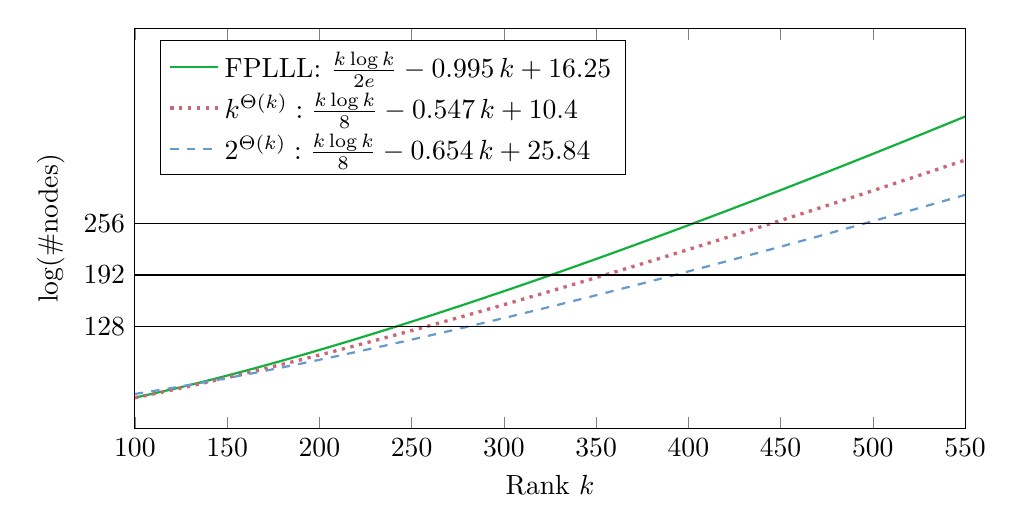
\begin{tikzpicture}
  \begin{axis}[
    legend pos = north west, 
    xlabel=Rank \(k\),
    xmin=100, xmax=550,
    ymin=0, ymax=500,
    height=0.55\textwidth,
    ylabel = \(\log(\#\textnormal{nodes})\),
    ytick = {128,192,256},
    ]
    \addplot+ [domain=100:550, samples=250]{0.1839*x*log2(x) - 0.995*x + 16.25};
    \addlegendentry{FPLLL: \(\frac{k \log k}{2e} - 0.995\,k + 16.25\)};

    \addplot+ [domain=100:550, samples=250]{0.125*x*log2(x) - 0.547*x+10.4};
    \addlegendentry{\(k^{\Theta(k)}: \frac{k \log k}{\alert{8}} - 0.547\,k + 10.4\)};

    \addplot+ [domain=100:550,samples=250]{0.125*x*log2(x) - 0.654*x+25.84};
    \addlegendentry{\(2^{\Theta(k)}: \frac{k \log k}{8} - \alert{0.654}\,k + 25.84\)};

    \addplot+ [domain=100:550, samples=200, solid, thin,draw=black]{128};
    \addplot+ [domain=100:550, samples=200, solid, thin,draw=black]{192};
    \addplot+ [domain=100:550, samples=200, solid, thin,draw=black]{256};
  \end{axis}
\end{tikzpicture}
\tikzset{external/export=false}
\end{frame}
\end{document}